%\newcommand\T{\rule{0pt}{2.6ex}}
%\newcommand\B{\rule[-1.2ex]{0pt}{0pt}}
%\newcommand\TT{\rule{0pt}{4.2ex}}
%\newcommand\BB{\rule[-2.4ex]{0pt}{0pt}}
%\newcommand\TTT{\rule{0pt}{3.8ex}}
\newcommand{\Ytwo}{{{}^{-2}Y}}

\newcommand\T{}
\newcommand\B{}
\newcommand\TT{}
\newcommand\BB{}
\newcommand\TTT{}



Thus far, most searches for gravitational waves from BBH mergers have
relied on post-Newtonian waveforms such as those discussed in
Sec.~\ref{sec:PNWaveforms}, which are valid when the black holes
are sufficiently far apart.  Within its range of validity,
post-Newtonian theory provides a convenient analytic description of
the expected signals produced by binary systems.  The numerical
relativity results, on the other hand, have not yet been synthesised
into an analytic model for the merger phase covering a broad range of
parameters, i.e., a wide range of mass ratios, spins and if necessary,
eccentricity; there has however been significant progress for the
non-spinning
case~\cite{Buonanno:2006ui,Berti:2007fi,Ajith:2007kx,Pan:2007nw,%
Buonanno:2007pf,Boyle:2007ft,%
Ajith:2007qp,Damour:2007yf,Damour:2007vq,Damour:2008te,Boyle:2008ge,Boyle:2009dg}.
Similarly, despite significant progress, there is not yet a complete
detailed description over the full parameter space of how
post-Newtonian and numerical simulations are to be matched with each
other.  On the data analysis side, many pipelines, especially ones
that rely on a detailed model for the signal waveform, have made a
number of choices based on post-Newtonian results, such as the use of
the Schwarzschild ISCO as a cutoff frequency, and it is important to
verify that these choices are sufficiently robust.  More generally, it
is necessary to quantify the performance of these data analysis
pipelines for both detection and parameter estimation.  This is
critical for setting astrophysical upper limits in case no detection
has been made, for following up interesting detection candidates, and
of course for interpreting direct detections.  Numerical relativity
now provides an important avenue for extending this beyond the early
inspiral phase captured by post-Newtonian waveforms, to the late
inspiral and merger phase.  

There are significant challenges to be overcome before numerical
relativity results can be fully exploited in data-analysis pipelines.
The Numerical INJection Analysis (NINJA) project was started in the
spring of 2008 with the aim of addressing these challenges and
fostering close collaboration between numerical relativists and data
analysts. Participation in NINJA is open to all scientists interested
in numerical simulations and gravitational-wave data analysis.  

Several decisions were make to limit the scope of the project.  NINJA
chose to restrict attention to BBH simulations and have not used
results from supernova simulations or simulations containing neutron
stars~\footnote{As of this writing a matter NINJA project is in an
early planning stage}.  For the first NINJA project (henceforth
``NINJA-1'') the waveform data came purely from numerical simulations
and we did not attempt to extend numerical data using post-Newtonian
waveforms.  The NINJA-1 data set was constructed using Gaussian noise
to model the response of the Initial LIGO and Virgo detectors --- no
attempt was made to include non-Gaussian noise transients found in
real detector data.  The comparisons and conclusions reported here are
thus necessarily limited, and in many cases are only the first steps
towards fully understanding the sensitivity of data-analysis pipelines
to black hole signals.  Further studies are needed regarding the
accuracy and comparison of numerical waveforms, and of how systematic
errors in these waveforms can affect parameter estimation.  Some
analyses of numerical waveforms with regard to gravitational-wave
detection have already been
performed~\cite{Baumgarte:2006en,Vaishnav:2007nm,Pan:2007nw,Boyle:2009dg},
accuracy standards have been developed for use of numerical waveforms
in data analysis~\cite{Lindblom:2008cm} and a detailed comparison of
some of the waveforms used in NINJA-1 was performed in the related
Samurai project~\cite{Hannam:2009hh}.  The NINJA-2 project, discussed
in the next chapter and currently ongoing at the time of writing, will
build on these results to begin to address these issues.  

Despite the limited scope of the NINJA-1, we are able to draw the
following broad conclusion from this work.  We conclude that the
current data analysis pipelines used to search LIGO, Virgo and GEO600
data for black hole coalescence are able to detect numerical waveforms
injected into the NINJA-1 data set at the expected sensitivities.
Indeed, the standard pipeline is able to detect signals that lie
outside the parameter space that they target.  This is a non-trivial
statement since most detectability estimates to date for these sources
have relied on post-Newtonian waveforms, which are valid only when the
black holes are sufficiently far apart.  It should be noted, however,
that the NINJA data set does not contain non-stationary noise
transients so more work is needed to understand how detection
performance is affected by the noise artifacts seen in real
gravitational-wave detector data.  NINJA has proven to be extremely
valuable at framing the questions that need to be answered.

% end introduction.tex

\section{Numerical Waveforms}
\label{sec:ninja1_nrwaveforms}
%begin nrwaveforms.tex

NINJA-1 studied BBH coalescence waveforms submitted by ten individuals
and teams.  Participation in NINJA-1 was open to anyone and the only
restrictions were that each contribution: (i) was a numerical solution
of the full Einstein equations, (ii) consisted of only two waveforms,
or up to five waveforms if they were part of a one-parameter family.

No restrictions were placed on the accuracy of each waveform. All
contributions followed the format specified in~\cite{Brown:2007jx}.
The waveforms are plotted in Figures~\ref{fig:NR-Reh22} and
\ref{fig:NR-SumAllModes}.
%
The contributed waveforms covered a variety of physical and numerical
parameters. Most simulations modeled low-eccentricity inspiral, the mass
ratio $q = m_1/m_2$ ranges from 1 to 4, and the simulations covered a
range of spin configurations.  The initial angular frequency of the
$\ell=m=2$ mode ranged from $0.033/M$ to $0.203/M$ (where $M$ denotes
the sum of the initial black-hole masses). This initial angular
frequency marks where contributors considered the waveform sufficiently
clean to represent the physical system (e.g. this will be chosen after
initial unphysical radiation content, often referred to as ``junk
radiation'' in numerical relativity, is radiated away).   The length
of the waveforms varied between a few 100M to over 4000M.  The
contributions naturally differed in accuracy, both regarding how well
they captured the black-hole dynamics and in the extraction of the
gravitational-wave signal. 

Table~\ref{tab:allwaveforms} lists a few key parameters that
distinguish the waveforms, and introduces the following tags for the
different contributions and codes:
%
% XXX This is the paragraph that people should copy to get the NINJA NR refs
%
BAM~HHB~\cite{Brugmann:2008zz,Husa:2007hp,Hannam:2007ik,Hannam:2007wf,Bruegmann:2003aw} 
and BAM~FAU~\cite{Brugmann:2008zz,Husa:2007hp,Tichy:2008du,Bruegmann:2003aw}
are contributions using the {\tt BAM} code,
{\tt CCATIE} is the AEI/LSU code~\cite{Alcubierre:2000xu,Alcubierre:2002kk,Koppitz:2007ev,Pollney:2007ss,Rezzolla:2007xa},
{\tt Hahndol} is the Goddard Space Flight Center's code~\cite{Imbiriba:2004tp,vanMeter:2006vi}, 
{\tt LazEv} is the RIT code~\cite{Zlochower:2005bj,Campanelli:2005dd,Dain:2008ck}, 
{\tt Lean} is Ulrich Sperhake's code~\cite{Sperhake:2006cy,Sperhake:2007gu, Sperhake2008},
{\tt MayaKranc} is the Georgia Tech/Penn State code~\cite{Vaishnav:2007nm,Hinder:2007qu}, 
PU stands for the Princeton University code~\cite{Pretorius:2004jg,Pretorius:2005gq,Buonanno:2006ui,Pretorius:2007jn},
{\tt SpEC} for the Cornell/Caltech collaboration 
code~\cite{Scheel:2006gg,Pfeiffer:2007yz,Boyle:2007ft,Scheel:2008rj},
and
{\tt UIUC} stands for the University of Illinois at
Urbana-Champaign team~\cite{Etienne:2007hr}.

The codes listed above use different formulations of the Einstein
equations, gauge conditions, mesh structures, initial data and wave
extraction methods.  Full details of each code are given in the
references.

% Refer back to chapter 3

\begin{table}
\begin{center}
\begin{tabular}{|l|l|l|l|l|l|c|c|}\hline
Code & Run & $q$ & $\vec S_i/m_i^2$ & $e$ & $\omega_{22}\, M$ & $D/M$ &
eccentricity
\\ 
\hfill Ref.     &     &   &                        &   &          &       &
     removal \\ \hline

BAM~FAU      & \cite{Tichy:2008du}       & 1 & 
%$\vec\chi_1^{\rm FAU}$,  $\vec\chi_2^{\rm FAU}$  
see caption
& qc  & 0.06 & $9.58\,\hat y$ & T-PN \cite{Marronetti:2007ya,Marronetti:2007wz} \\
\hfill\cite{Brugmann:2008zz,Husa:2007hp}              &        &   &
&    &      & &   \\[1em]

BAM~HHB      & S00 \cite{Hannam:2007ik}   & 1 & $0$       & $< 0.002$   &
0.045 & $12\,\hat y$ & TR-PN \cite{Husa:2007rh} \\ 
\hfill\cite{Brugmann:2008zz,Husa:2007hp}              & S25 \cite{Hannam:2007wf}   & 1 & $0.25\,\hat z$    & $\approx 0.006$  &
              0.045 & $12\,\hat y$ & T-PN \cite{Brugmann:2007zj} \\
              & S50 \cite{Hannam:2007wf}   & 1 & $0.50\,\hat z$    & $\approx 0.006$  &
              0.052 & $11\,\hat y$ & -- '' -- \\ %T-PN \cite{Brugmann:2007zj} \\
              & S75 \cite{Hannam:2007wf}   & 1 & $0.75\,\hat z$    & $\approx 0.006$ &
              0.06 &  $10\,\hat y$ & -- '' -- \\ %T-PN \cite{Brugmann:2007zj} \\
              & S85 \cite{Hannam:2007wf}   & 1 & $0.85\,\hat z$    & $\approx 0.006$  &
              0.06 &  $10\,\hat y$ & -- '' -- \\[1em] %T-PN
                                %\cite{Brugmann:2007zj} \\


{\tt CCATIE}
              & r0~\cite{Pollney:2007ss}    & 1 & $0.6\,\hat z$, $-0.6\,\hat z$  & qc &
              0.079 & $8\,\hat x$ & TR-PN \cite{Husa:2007rh} \\
\hfill\cite{Alcubierre:2000xu,Alcubierre:2002kk,Koppitz:2007ev,Pollney:2007ss}
	      & r2~\cite{Pollney:2007ss}     & 1 & $0.6\,\hat z$, $-0.3\,\hat z$    & qc  &
              0.078 & $8\,\hat x$ & -- '' -- \\ %TR-PN \cite{Husa:2007rh} \\
              & r4~\cite{Pollney:2007ss}     & 1 & $0.6\,\hat z$, $0$       & qc  &
              0.076 & $8\,\hat x$ & -- '' -- \\ %TR-PN \cite{Husa:2007rh} \\
              & r6~\cite{Pollney:2007ss}     & 1 & $0.6\,\hat z$, $0.3\,\hat z$    & qc  &
              0.075 & $8\,\hat x$ & -- '' -- \\%TR-PN \cite{Husa:2007rh} \\
              & s6~\cite{Rezzolla:2007xa}     & 1 & $0.6\,\hat z$     & qc  &
              0.074 & $8\,\hat x$ & -- '' -- \\[1em] %TR-PN \cite{Husa:2007rh} \\ 
  \hline
\end{tabular}
\end{center}
\caption[Initial conditions for numerical waveforms.]{
\label{tab:allwaveforms}
Initial conditions for numerical waveforms.
The columns list: 
the name of the contribution, the name of the run
if appropriate, 
the mass ratio $q=m_1/m_2$ where $m_1\ge m_2$, the
spins of the black holes (if only one spin is given, both spins are equal), an estimate of the initial
eccentricity of the orbit (``qc'' denotes cases where quasi-circular inspiral 
is modelled, but a value of the eccentricity has not been reported), the initial frequency of the $(2,2)$
mode (rounded to three digits), the initial coordinate separation
of either the black-hole punctures or the excision surfaces, and where
appropriate the method of eccentricity removal.  All binaries start
 in the $xy$-plane with momenta tangent to the $xy$-plane.  See text for the
identification of each contribution, and a description of the notation
in the last column. 
The dimensionless spins of the BAM~FAU run are $(-0.634,-0.223, 0.333)$ and 
$(-0.517,-0.542,0.034)$.}
\end{table}



\begin{table}
\begin{center}
\begin{tabular}{|l|l|l|l|l|l|c|c|}\hline
Code & Run & $q$ & $\vec S_i/m_i^2$ & $e$ & $\omega_{22}\, M$ & $D/M$ &
eccentricity
\\ 
\hfill Ref.     &     &   &                        &   &          &       &
     removal \\ \hline
{\tt Hahndol}      & kick   & 3 & $0.2\,\hat x$, $0.022\,\hat x$ & qc  &0.078 &  $8.007\,\hat{y}$ & T-PN \cite{Kidder:1995zr}\\ 
\hfill\cite{Imbiriba:2004tp,vanMeter:2006vi}            & non    & 4 & $0$     & qc
              &0.070 & $8.470\,\hat{y}$ & -- '' -- \\ %T-PN \cite{Kidder:1995zr} \\

{\tt LazEv}$\,$\cite{Zlochower:2005bj,Campanelli:2005dd}$\!$    & MH~\cite{Dain:2008ck} & 1 & $0.92\,\hat z$   & qc  &
0.07  & $8.16\,\hat x$ & T-PN \cite{Kidder:1995zr,Blanchet:1999pm} \\[1em]

{\tt Lean}\hfill\cite{Sperhake:2006cy}      &  c     & 4 & $0$       & qc  &
0.05  & $10.93\,\hat x$ & T-PN \cite{Brugmann:2008zz} \\ 
             &  2     & 1 & $0.926\,\hat z$   & qc  &
              0.11  & $6.02\,\hat x$ & T-PN \cite{Kidder:1995zr} \\[1em]

{\tt MayaKranc}     & e0  \cite{Hinder:2007qu}   & 1 & $0$       &  qc &
0.05 & $12\,\hat x$ & TR-PN \cite{Husa:2007rh} \\
  \hfill\cite{Vaishnav:2007nm}            & e02 \cite{Hinder:2007qu}   & 1 & $0$       & 0.2&
              0.05 & $15.26\,\hat x$ & n/a \\[1em]

PU\hfill\cite{Pretorius:2004jg,Pretorius:2005gq}  & CP \cite{Buonanno:2006ui}    & 1 & $0.063\,\hat z$      & qc  &
0.07  & $9.5\,\hat x$ & T-ID \cite{Cook:2004kt} \\
              & T52W \cite{Pretorius:2007jn}  & 1 & $0$       & $\ge
              0.5$ & 0.07 & & n/a \\[1em]

{\tt SpEC}\hfill  \cite{Scheel:2006gg}        & q=1 \cite{Boyle:2007ft,Scheel:2008rj}       & 1 & $0$       & $5\times 10^{-5}$  &
0.033 & $15\,\hat x$ & TR-it \cite{Pfeiffer:2007yz} \\[1em]

UIUC \hfill\cite{Etienne:2007hr}          & cp \cite{Etienne:2007hr}     & 1 & $0$       & qc  &
0.194 & $4.790\,\hat x$ & T-ID \cite{Cook:2004kt} \\ 
             & punc \cite{Etienne:2007hr}   & 1 & $0$     & qc  &
              0.203 & $4.369\,\hat y$ & T-ID \cite{Tichy:2003qi} \\ 

 \hline
\end{tabular}
\end{center}
\caption[Initial conditions for numerical waveforms.]{
\label{tab:allwaveforms}
Initial conditions for numerical waveforms.
The columns list: 
the name of the contribution, the name of the run
if appropriate, 
the mass ratio $q=m_1/m_2$ where $m_1\ge m_2$, the
spins of the black holes (if only one spin is given, both spins are equal), an estimate of the initial
eccentricity of the orbit (``qc'' denotes cases where quasi-circular inspiral 
is modelled, but a value of the eccentricity has not been reported), the initial frequency of the $(2,2)$
mode (rounded to three digits), the initial coordinate separation
of either the black-hole punctures or the excision surfaces, and where
appropriate the method of eccentricity removal.  All binaries start
 in the $xy$-plane with momenta tangent to the $xy$-plane.  See text for the
identification of each contribution, and a description of the notation
in the last column.} 
\end{table}



\begin{table}
\begin{center}
\begin{tabular}{|l|l|c||c|c|c|}\hline
Code & Run & q % & $\vec S_i/m_i^2$ & e & $\omega_{22}\, M$ 
& $\Delta T_{\rm 100}$ [s] & $f_{i,\rm 100}$ [Hz] & $M_{30 Hz} [M_\odot]$ \\ %& ${\cal M}_{30 Hz} [M_\odot]$
 \hline

BAM~HHB    & S00  & 1 % & $0$                   & $< 0.002$ & 0.045 
& 1.03 & 15 & 48  \\ %& 21 \\ 
            & S25  & 1 % & $0.25\hat z$  & $\approx 0.006$  & 0.045 
& 1.15 & 15 & 48  \\ %& 21 \\
            & S50  & 1 % & $0.50\hat z$  & $\approx 0.006$  & 0.052 
& 1.03 & 17 & 56  \\ %& 24 \\
            & S75  & 1 % & $0.75\hat z$  & $\approx 0.006$  & 0.06  
& 0.81 & 19 & 65  \\ %& 28 \\
            & S85  & 1 % & $0.85\hat z$  & $\approx 0.006$  & 0.06  
& 0.87 & 19 & 65  \\ %& 28 \\

BAM~FAU    &      & 1 % & see caption                   & qc & 0.06  
& 0.54 & 19 & 65  \\ %& 28 \\ 

{\tt CCATIE}& r0   & 1 % & $0.6\hat z$, $-0.6\hat z$ & qc & 0.079 
& 0.34 & 26 & 85  \\ %& 37\\
            & r2   & 1 % & $0.6\hat z$, $-0.3\hat z$ & qc & 0.078 
& 0.37 & 25 & 84  \\ %& 37 \\
            & r4   & 1 % & $0.6\hat z$, $0$            & qc & 0.076 
& 0.40 & 25 & 82  \\ %& 36 \\
            & r6   & 1 % & $0.6\hat z$, $0.3\hat z$  & qc & 0.075 
& 0.45 & 24 & 81  \\ %& 35 \\
            & s6   & 1 % & $0.6\hat z$                 & qc & 0.074 
& 0.59 & 24 & 80  \\ %& 35 \\

{\tt Hahndol}&kick & 3 % & $0.2\hat x$, $0.022\hat x$& qc & 0.078 
& 0.25 & 25 & 84  \\ %& 31 \\
            & non  & 4 % & $0$                           & qc & 0.070 
& 0.32 & 23 & 75  \\ %& 25 \\

{\tt LazEv} & MH   & 1 % & $0.92\hat z$                & qc & 0.07  
& 0.43 & 23 & 75  \\ %& 33 \\

{\tt Lean}  &  c   & 4 % & $0$                           & qc & 0.05  
& 0.92 & 16 & 54  \\ %& 18 \\
            &  2   & 1 % & $0.926\hat z$               & qc & 0.11  
& 0.20 & 36 & 118\,\,\,  \\ %& 52 \\

{\tt MayaKranc}& e0& 1 % & $0$                           & qc & 0.05  
& 1.23 & 16 & 54  \\ %& 23 \\
            & e02  & 1 % & $0$                          & 0.2 & 0.05  
& 0.74 & 16 & 54  \\ %& 23 \\

PU          & CP   & 1 % & $0.063\hat z$               & qc & 0.07  
& 0.29 & 23 & 75  \\ %& 33 \\
            & T52W & 1 % & $0$                   & $\ge  0.5$ & 0.07  
& 0.16 & 23 & 75  \\ %& 33 \\

{\tt SpEC}  & q=1  & 1 % & $0$                   & $<10^{-5}$  & 0.033 
& 1.96 & 11 & 36  \\ %& 15 \\

UIUC        & cp   & 1 % & $0$                           & qc & 0.194 
& 0.10 & 63 & 209\,\,\,  \\ %& 91 \\
            & punc & 1 % & $0$                           & qc & 0.203 
& 0.10 & 66 & 219\,\,\,  \\ %& 95 \\

 \hline
\end{tabular}
\end{center}
\caption[Characteristic duration, mass and frequencies of the NINJA-1
submissions]{
\label{tab:allwaveforms-SI}
Characteristic duration, mass and frequencies of
the waveforms summarised in table~\ref{tab:allwaveforms}.
The columns $\Delta T_{\rm 100}$ and $f_{i, 100}$ give the duration and initial
frequency of the waveform when scaled to total mass $M=100M_{\odot}$.
$M_{30Hz}$ is the total mass of the waveform when it is scaled so that
the initial frequency is 30Hz (this sets the lowest mass at which each waveform  can be injected into the NINJA data).}
\end{table}



%%%%%%%%%%%%%%%%%%%%%%%%%%%%%%%%%%%%%%%%%%%%%%%%%%%%%%%%%%%%%%%%

\begin{figure}
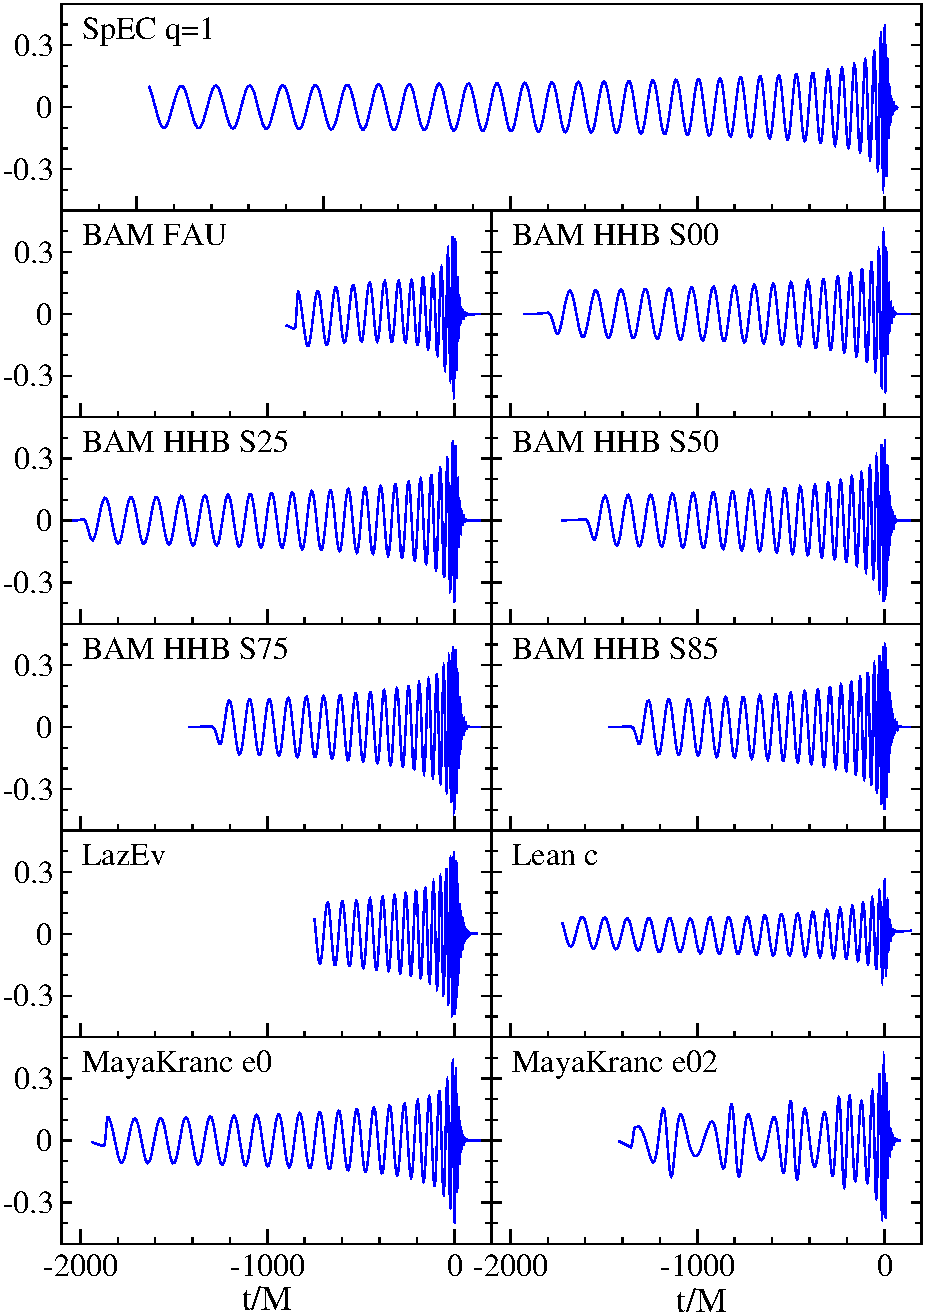
\includegraphics[width=0.49\textwidth]{figures/ninja1/Prune_Re_h22-A}
$\;$
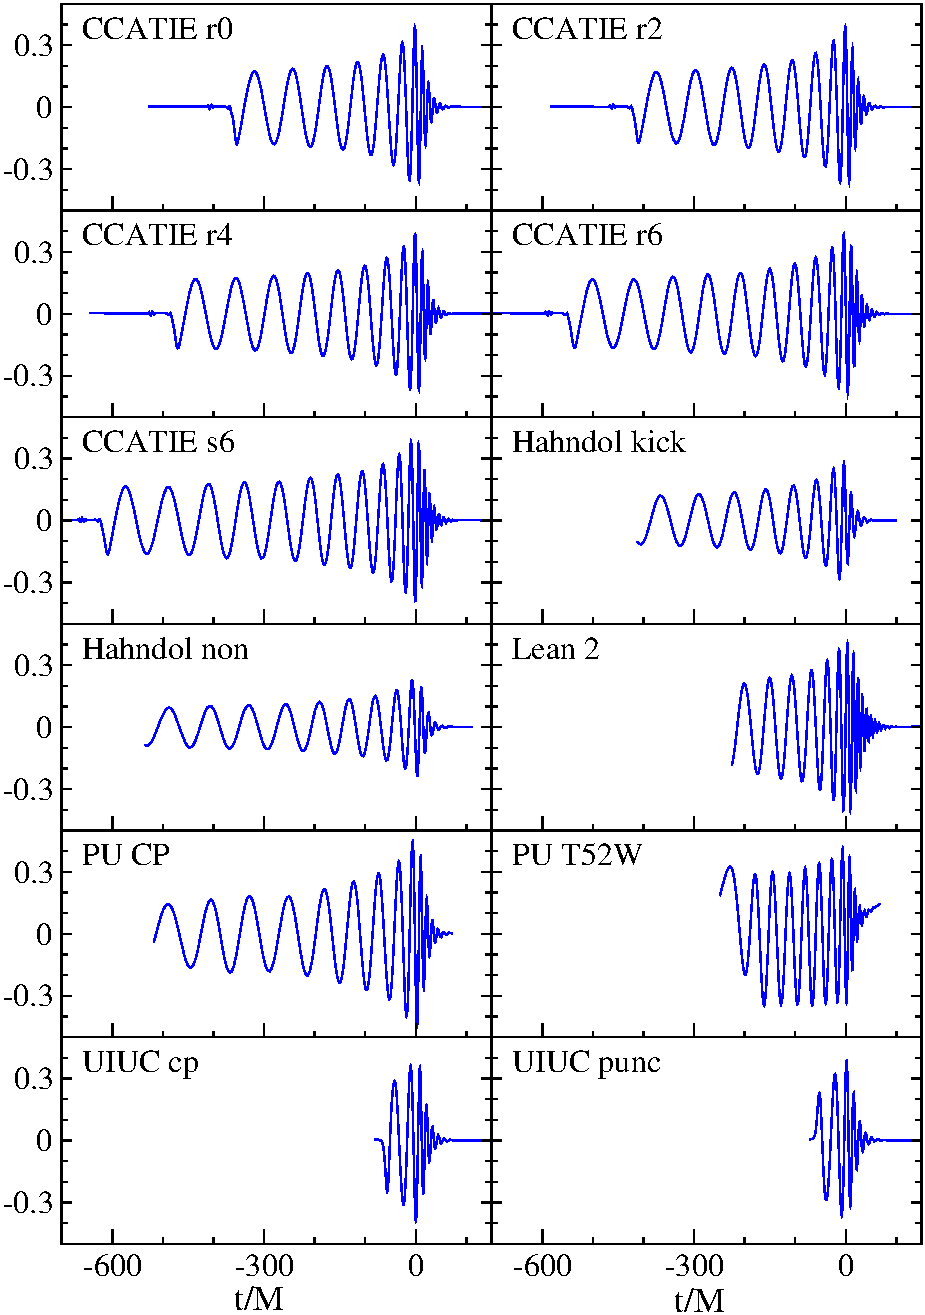
\includegraphics[width=0.49\textwidth]{figures/ninja1/Prune_Re_h22-B}\\[-.25em]

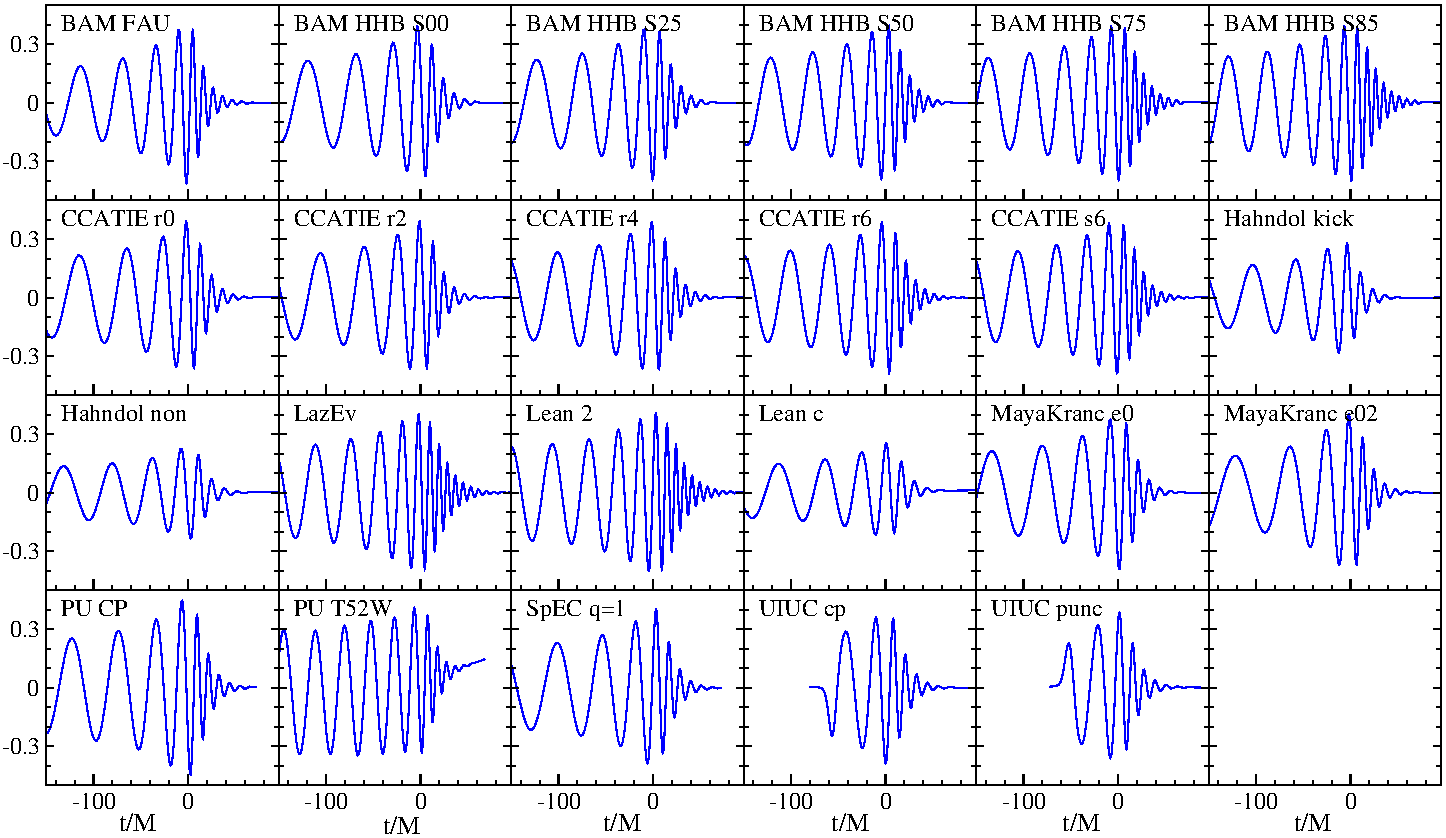
\includegraphics[width=\textwidth]{figures/ninja1/Prune_Re_h22-Merger}
\caption[Summary of waveforms contributed to NINJA-1]{
\label{fig:NR-Reh22}
Summary of all submitted numerical waveforms:
\boldmath$r/M\,\mbox{Re}(h_{22})$ The $x$-axis shows time in units of
$M$ and the $y$-axis shows the real part of the $(\ell,m)=(2,2)$
component of the dimensionless wave strain $r h = r h_+ - i r
h_\times$.  The top panels show the complete waveforms: the top-left
panel includes waveforms that last more than about $700M$, and the
top-right panel includes waveforms shorter than about $700M$. The
bottom panel shows an enlargement of the merger phase for all
waveforms.}
\end{figure}


\begin{figure}
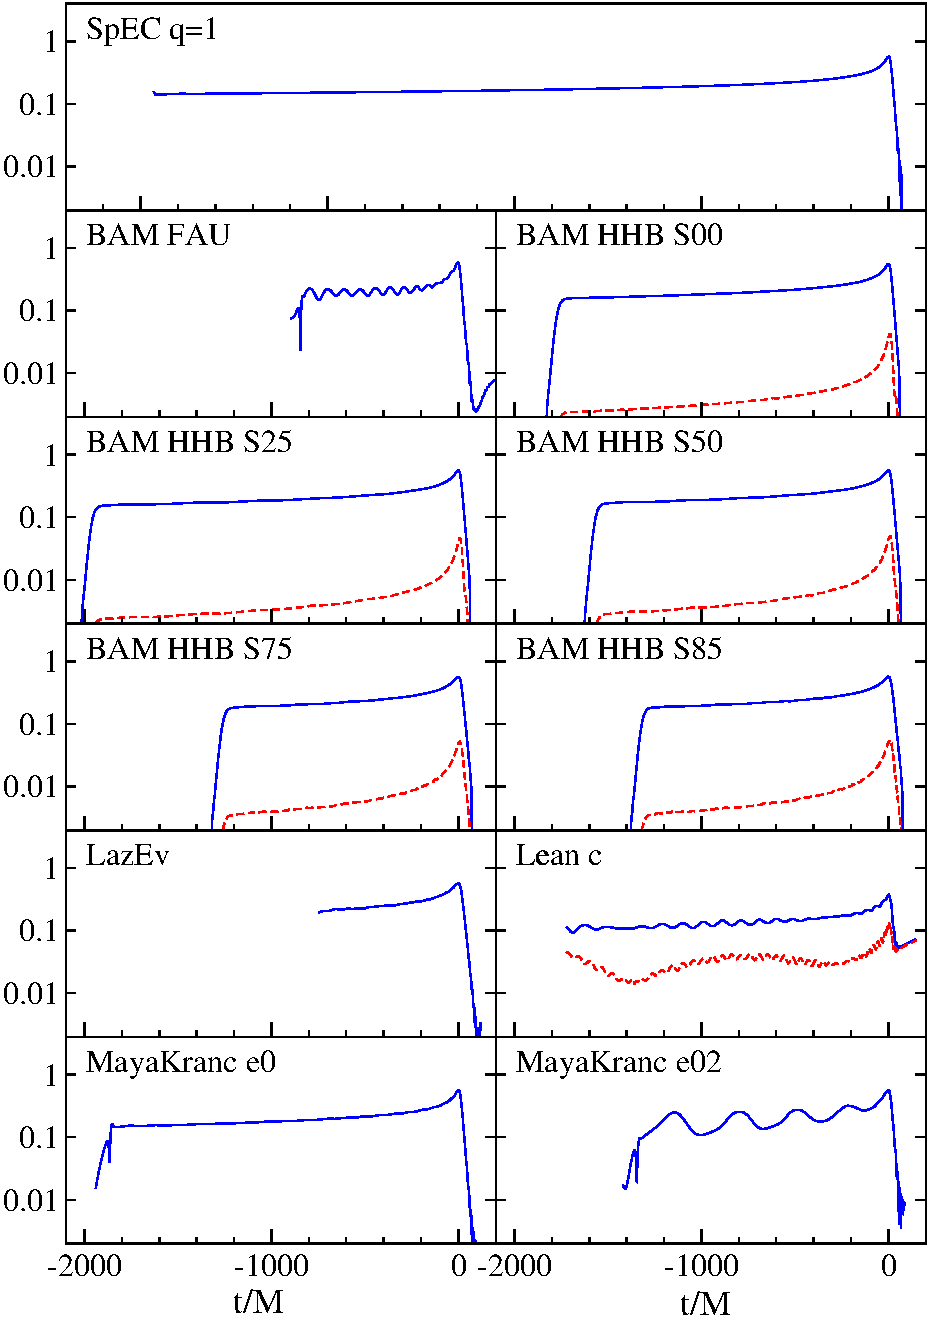
\includegraphics[width=0.49\textwidth]{figures/ninja1/Prune_SumAllModes-A}
$\;$
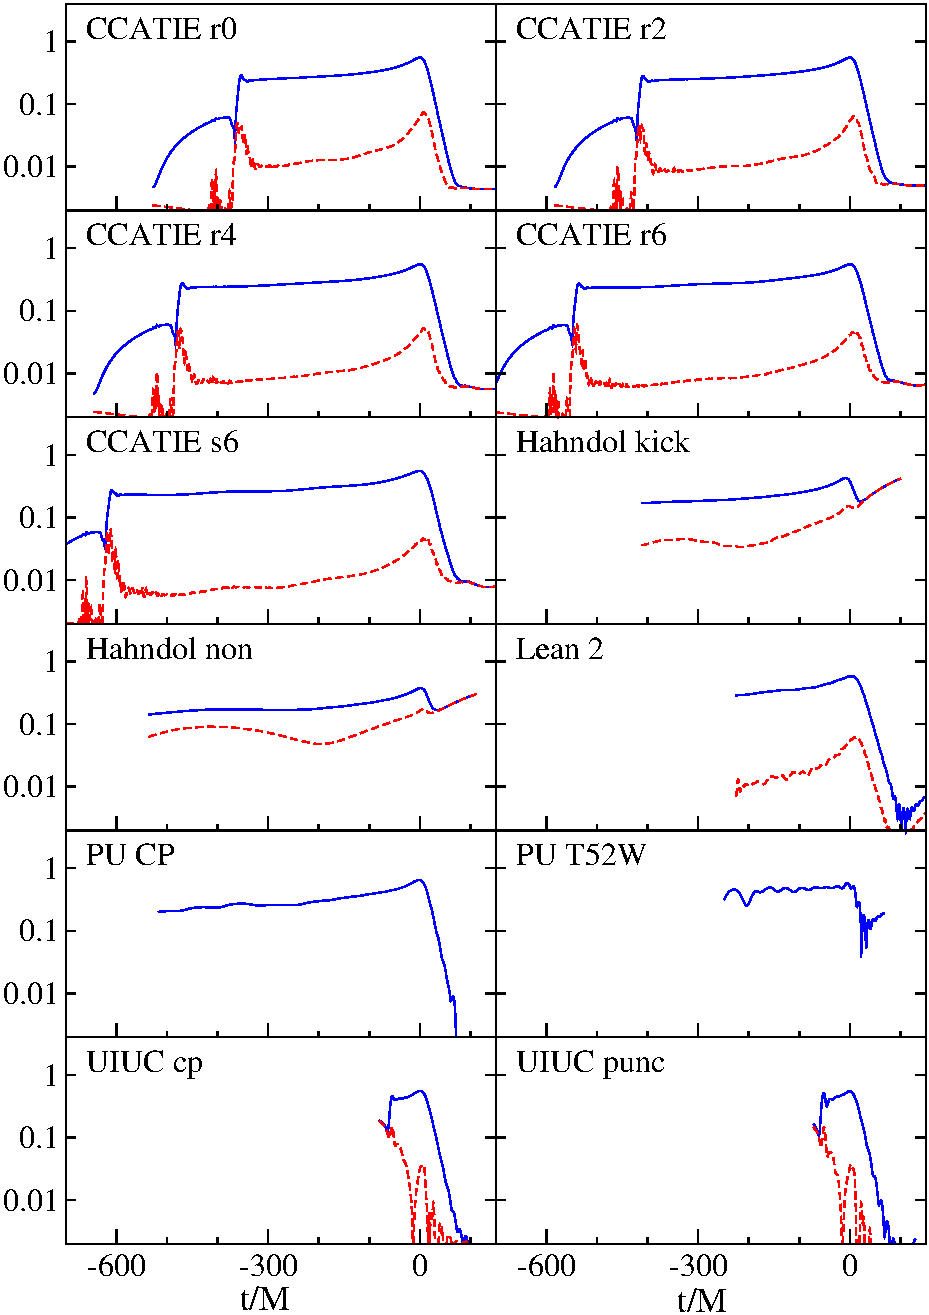
\includegraphics[width=0.49\textwidth]{figures/ninja1/Prune_SumAllModes-B}\\[-0.25em]

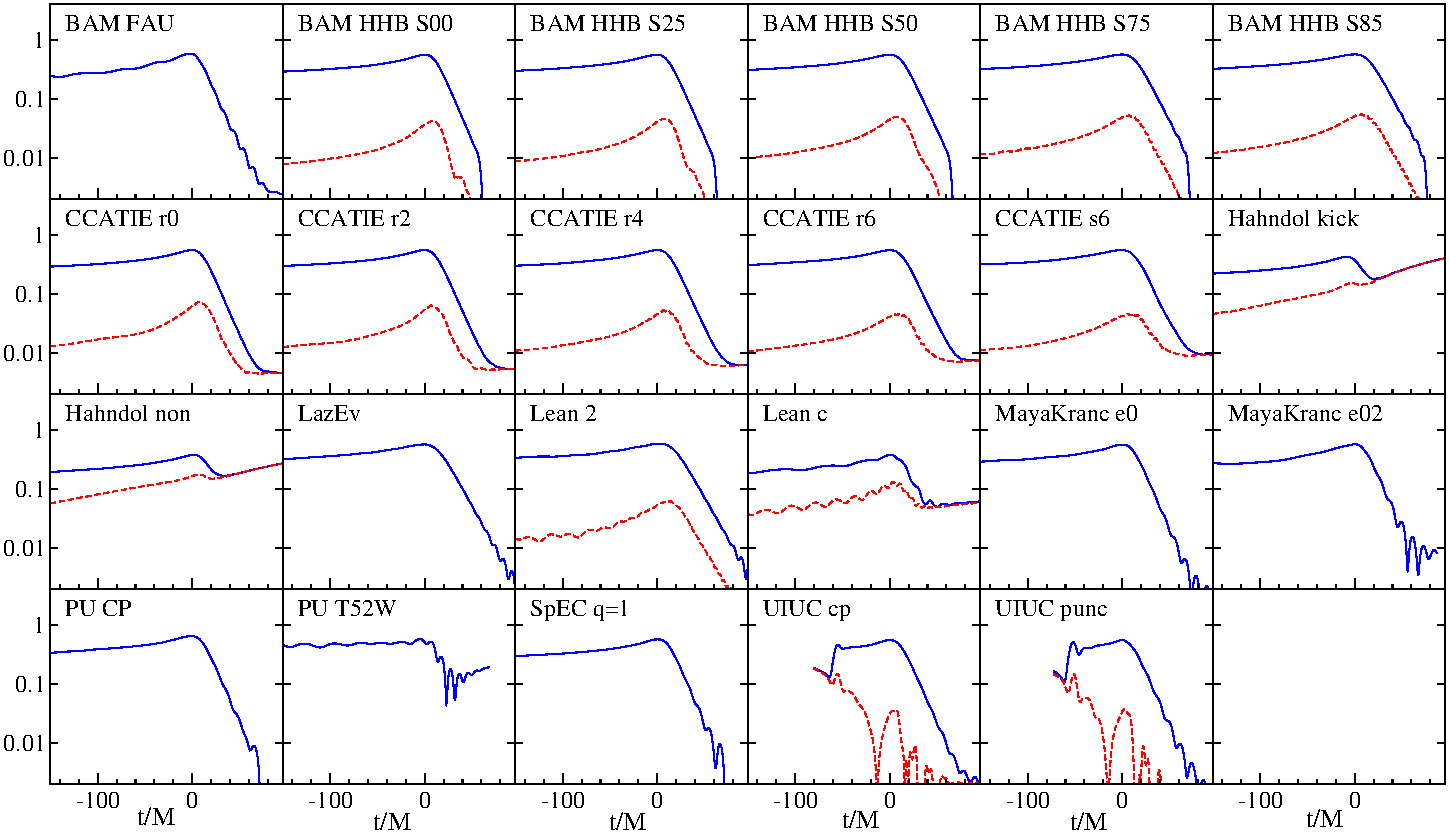
\includegraphics[width=\textwidth]{figures/ninja1/Prune_SumAllModes-Merger}

\caption[Distribution of power into different spherical harmonics]{
\label{fig:NR-SumAllModes}
Distribution of power into different spherical harmonics.  The blue line shows
  $\left(\Sigma_{\ell,m}|h_{\ell m}\,r/M|^2\right)^{1/2}$.  A dashed red line, if
  present, shows the same sum, but {\em excluding} the $(\ell,m)=(2,\pm
  2)$ modes. 
  The separation between the two lines gives the relative importance
  of non $(2,\pm 2)$ modes.  If no red line is present for a certain
  run, then only the $(2,\pm 2)$ modes were supplied.  The layout is
  as in Fig.~\ref{fig:NR-Reh22}: The top panels show the complete
  waveforms, whereas the bottom panel shows an enlargement of the
  merger phase. The $x$-axis shows time in units of $M$.
}
\end{figure}

\iffalse
The numerical codes follow either of two approaches to solving the
Einstein equations: (1) the generalised harmonic formulation, which
was the basis of Pretorius' initial breakthrough simulation of
coalescing black holes \cite{Pretorius:2005gq}, or (2) the
moving-puncture approach, following
\cite{Campanelli:2005dd,Baker:2005vv}.  Both approaches result in
canonical choices for the construction of initial data, the evolution
system for the Einstein equations, and the treatment of the
singularity inside the black-hole horizons.
%%%%%%%%%%%%%%%%%%%%%%%%%%%%%%%%%%%%%%%%%%%%%%%%%%%%%%%%%%%%%%%%%%%%%%%


%%%%%%%%%%%%%%%%%%%%%%%%%%%%%%%%%%%%%%%%%%%%%%%%%%%%%%%%%%%%%%%%%%%%%%%
\subsection{Summary of the Simulation Algorithms}
\label{ssec:sumalg}

%%%%%%%%%%%%%%%%%%%%%%%%%%%%%%%%%%%%%%%%%%%%%%%%%%%%%%%%%%%%%%%%%%%%%%%
\subsubsection{Initial Data}
\label{ssec:id}

Due to the presence of constraint equations, specifying initial data
in numerical relativity is far from trivial, for a general overview
see e.g.~\cite{Cook:2000vr}.  All of the results presented here make
the simplifying assumption of conformal flatness for the spatial
metric of the initial slice, which leads to some spurious
gravitational radiation in the initial data.  All contributions
attempt to model non-eccentric inspiral, except for the two data sets
PU--T52W and {\tt MayaKranc}--e02.  However, the degree of
``quasi-circularity'' varies, and in general one should bear in mind
that the definition of eccentricity for fully general-relativistic
orbits is not unique (see for
example~\cite{Sperhake:2007gu,Hinder:2007qu}).   The data set PU--T52W
is notable for the fact that the BBH was constructed via scalar field
collapse. Specifically, the initial data consists of two, compact,
dense distributions of scalar field energy, separated by some distance
and Lorentz boosted in opposite directions orthogonal to the line
between them. Upon subsequent evolution, each scalar field pulse
quickly collapses to form a black hole, with all remnant scalar field
energy radiating away from the domain on the order of the
light-crossing time of the orbit. This is the same time scale on which
spurious gravitational radiation present in all current initial-data
sets leaves the domain of the inspiral, and hence for practical
purposes this can be considered a vacuum merger.  All other runs start
from vacuum initial data. 

Most codes ({\tt BAM}, {\tt CCATIE}, {\tt Hahndol}, {\tt LazEv}, {\tt
Lean}, {\tt MayaKranc} and the UIUC code) adopt the ``moving
puncture'' approach, following \cite{Campanelli:2005dd,Baker:2005vv}.
These codes use puncture initial data
\cite{Bowen:1980yu,Beig:1993gt,Brandt:1997tf} to model black holes,
resulting in initial data that contain a separate asymptotically flat
end within each black hole.  Constructing such initial data is
mathematically well understood~\cite{Beig:1993gt,Dain:2001ry}. 
% I think the next sentence is misleading, if you really want to have
% it in, contact me please - Sascha.  and for simple cases the
% evolution of such initial data has been shown to be equivalent to
% that of excised black holes~\cite{Thornburg:2007hu}.
The codes {\tt CCATIE}, {\tt LazEv}, {\tt Lean} and {\tt MayaKranc}
all use the same pseudo-spectral solver for the Einstein constraint
equations~\cite{Ansorg:2004ds}, and {\tt BAM} uses a variant
thereof~\cite{Husa:2007hp}.  {\tt UIUC-punc} initial data is generated
via the \textsc{Lorene} \cite{Lorene} multi-domain spectral libraries.
The {\tt Hahndol} code uses the second-order-accurate multi-grid
solver \textsc{amrmg} \cite{Brown:2004ma}, which is however tuned to
give truncation errors typically much smaller than those produced by
the evolution code.

The generalised harmonic codes use conformal thin sandwich initial
data~\cite{York:1998hy}.  PU-CP and {\tt SpEC} use quasi-equilibrium
excision initial data  where the interior of the black-hole horizons
has been excised from the numerical grid. The presence of black holes
with desired linear momenta and spins is enforced through the boundary
conditions on the excision surfaces and the numerical outer boundary
during the solution of the initial-value equations
\cite{Cook:2001wi,Cook:2004kt,Caudill:2006hw,Pfeiffer:2007yz}. This
``excision technique'' is based on the defining property of black
holes --- the horizons act as causal membranes and information cannot
escape from the inside.  The {\tt UIUC-cp} simulation uses the same
excised initial data, but fills the BH interior with ``smooth junk'',
as described in~\cite{Etienne:2007hr}, before evolving with the moving
puncture technique.   
% This is a repeat of the material above:
%PU--T52W uses initial data in which black holes are formed by scalar
%field collapse. 

All codes take input parameters that ultimately determine the
individual black-hole masses $m_i$, spins $\vec{S}_i$, momenta
$\vec{P}_i$ and coordinate separation $D$ of the black holes (one
should however be aware that in the strong field regime of general
relativity various subtleties are associated with the definition of
all of these quantities). In addition, the black-hole masses and
dimensionless spins slowly change during the inspiral, which requires
additional caution regarding the definition and accuracy of the values
of mass, spin, etc.  There are two common methods to estimate the
instantaneous individual black-hole masses. One is to calculate the
\emph{apparent-horizon mass}, computed from the irreducible mass
(given by the area of each hole's horizon) and the spin according to
Christodoulou's \cite{Christodoulou:1970wf} relation $m_i^2 =
m_{i{\rm,irr}}^2 + S_i^2/(4 m_{i,{\rm irr}}^2)$. The other, applicable
only to puncture data, is to compute the Arnowitt-Deser-Misner (ADM)
mass~\cite{Arnowitt1962} at each puncture, which corresponds to
spatial infinity in a space that contains only that black
hole~\cite{Brandt:1997tf}. We generally use the total black-hole mass
$M=m_1+m_2$ to scale dimensionful quantities, although sometimes the
total conserved energy ($M_\mathrm{ADM}$) is used for this purpose. 
%
% There are essentially two different approaches to quoting
% mass-related parameters of the black holes. One approach (e.g.\
% Goddard) is to assume that all the Bowen-York spin is ultimately
% absorbed by its puncture (this usually takes $\sim 30 M$ to happen).
% From these horizon masses, we calculate the symmetric mass ratio
% $\eta \equiv m_1 m_2/(m_1+m_2)^2$.  This gives the most precise
% specification of the actual mass ratio attained in our simulations.
% Another (used e.g.\ for the BAM~HHB contribution) is to take these
% parameters from the post-Newtonian initial parameters that are used
% to initialize a simulation. 
%
Without loss of generality all codes chose the rest frame where $\vec
P_1 = -\vec P_2$ and, thus, the net linear momentum vanishes
initially.     
%
% Note that we will not make a systematic distinction of whether
% quoted masses are directly determined from the horizon, or by some
% other method, e.g., through an identification with a post-Newtonian
% configuration, as these differences are usually found to be rather
% small, and the present work does not aim at the estimation of
% parameters with high precision. 

Those simulations that attempt to model non-eccentric inspiral use
initial parameters calculated by a number of different methods. Ideal
initial parameters would produce tangential motion consistent with
circular orbits, and radial motion consistent with slow inspiral. The
various methods to choose initial parameters can be broadly
characterised as those that attempt to provide only tangential motion
(so that initially the black holes have no radial momenta), denoted by
``T'' in the last column of Tab.~\ref{tab:allwaveforms}, and those
that provide both tangential and radial motion (denoted by ``TR'').
The procedures to estimate these parameters are based on properties of
the initial-data set (``ID''), post-Newtonian methods (``PN''), or an
iterative procedure following the results of several trial simulations
(``it''). In Tab.~\ref{tab:allwaveforms} we indicate which of these
variants was used, and provide a reference to the specific algorithm;
for the post-Newtonian methods in particular there are several
variants.  Note that the estimates of the resulting eccentricity range
from $e\sim 5\times 10^{-5}$ (for the {\tt SpEC} contribution) up to
$e \sim 0.02$. 

The two data sets from the UIUC contribution actually compare two {\em
alternative} sets of non-spinning, equal-mass, quasi-circular initial
data, with initial orbital frequency $M\Omega=0.0824$: (i) Puncture
initial data with coordinate separation $D/M=4.369$ and initial linear
momentum of each BH set according to \cite{Tichy:2003qi}, and (ii)
Cook-Pfeiffer initial data with coordinate separation $D/M=4.790$
\cite{Pfeiffer_data,Cook:2004kt} (measured from the centroids of the
apparent horizons), filling the BH interior with data that smoothly
connect to the exterior as described in \cite{Etienne:2007hr}.  Both
data sets yield the same final spin $\vert\vec S_{BH}\vert/M_{BH}^2 =
0.68$, but differ at the level of a few percent in radiated energy and
angular momentum. 
%\begin{table}[h]\label{tab:uiuc} \begin{center}
%\begin{tabular}{c|ccc} \hline & $\Delta E/M$ & $\Delta J/J$ &
%$J_{BH}/M_{BH}^2$ \\ \hline Puncture      & 0.028 & 0.21 & 0.68 \\
%Cook-Pfeiffer & 0.030 & 0.22 & 0.68 \\ \hline \end{tabular} \caption{
%radiated energy and angular momentum, and final spin for the two
%cases.} \end{center} \end{table}

For the eccentric {\tt MayaKranc} simulation (data set e02), the
conservative, third-post-Newtonian-order (3PN) expressions in
Ref.~\cite{Konigsdorffer:2006zt} have been used to specify initial
data.  These expressions require the specification of the eccentricity
$e$ and the mean motion $n = 2\pi/T_r$, where $T_r$ is the radial
(pericenter to pericenter) orbital period.  There are three PN
eccentricities, which are the same to 1PN order, and we choose $e_t$,
which appears in the PN Kepler equation, following
Ref.~\cite{Konigsdorffer:2006zt}.  The quantity $n$ has been chosen as
$n = 0.01625/M$ ($T_r \sim 387 M$) and $e=0.2$.  The binary
separation, $D/M=15.264$, was determined from Eqn.~(23) in
Ref.~\cite{Konigsdorffer:2006zt}, and the tangential linear momentum,
$P/M$=0.0498, of each black hole at apocenter was obtained from $J = P
D$, where $J$ is the total angular momentum computed as a
post-Newtonian expansion in $n$ and $e$ (Eqn.~(21) in
Ref.~\cite{Konigsdorffer:2006zt}).

%Please note that the eccentricity we are quoting can be taken only as
%a guide to the eccentricity in the initial data, as the post-Newtonian
%expressions used do not include radiation reaction, and the
%post-Newtonian parameters are in a different coordinate system to the
%puncture initial data.



%%%%%%%%%%%%%%%%%%%%%%%%%%%%%%%%%%%%%%%%%%%%%%%%%%%%%%%%%%%%%%%%%%%%%%%
\subsubsection{Evolution Systems}
\label{ssec:ev}

There is a long history of casting the Einstein equations into systems
of partial differential equations, and in 
particular into the form of a well-posed initial value problem. The
process of writing the covariant Einstein equations 
in the form of three-dimensional tensor quantities that evolve in time
is commonly referred to as a 3+1 split. The fundamental idea
is to choose coordinates $\{x^{i},t\}$ $(i=1,2,3)$ such 
that the spacetime metric can be written in the form
\begin{equation}
\label{3+1_split}
ds^2 = -(\alpha^{2}-\gamma_{ij}\beta^{i}\beta^{j})dt^{2}
   + 2 \gamma_{ij}\beta^{j}dt\,dx^{i}
   + \gamma_{ij}dx^{i}\,dx^{j}, 
\end{equation}
where $\gamma_{ij}$ is a positive-definite metric on the slices of
constant time $t$, and the scalar function $\alpha$ and  
vector field $\beta^i$ are commonly used to encode the freedom of
coordinate choice. They may in principle be freely specified, but in
practice they are judiciously prescribed, usually through further evolution equations.

%%%%%%%%%%%%%%%%%%%%%%%%%%%%%%%
\begin{table}
\begin{center}
\begin{tabular}{|c|c|c|c|c|c|c|c|}\hline
Code        & $\!$System$\!$ & $\!$Technique$\!$   & shift   &  $M \eta$ & $r_{max}/M$ & $r_{ext}/M$ & \TTT \BB $\displaystyle\frac{h_{min}}{0.001M}$   
\\\hline

BAM~HHB   & BSSN  &  FD--6         & 000 & 2         &  $773$      & $90$        & 56, 19 \\ %\{$3\times M/53.3$, \\ 
%&            &            &         &           &            &             & $2\times M/106.7$\} \\

BAM~FAU   & BSSN &  FD--6         & 000 & 2         &  $436$      &  $50$        & $16$\\ %$M/64$        \\ 

{\tt CCATIE}   & BSSN   &  FD--4         & 000 & 1         &  $819$    & $160$   & 20      \\

{\tt Hahndol} & BSSN    &  FD--$4,6$         & 000 &  2        &  $> 1000$   & $45$        & 19, 13 \\% $M/160$ to        \\
%&            &            &         &           &            &             & $3M/224$   \\

{\tt LazEv}   & BSSN &  FD--4         & ttt & 6         &  1281      & $40$            &   3.1 \\ % $M/320$      \\ 

{\tt Lean}   & BSSN     &  FD--$4,6$ & 000 &  1.25,1     &  $153.6$, $256$   & $60$, $61$         & 19, 13 \\ %\{1/52, 1/80\}        \\

{\tt MayaKranc} & BSSN  &  FD--4         & 000 & 2         &  $317.4$     & $70$            & 16, 19 \\ %\{$M/64.5$, $M/51.6$\}         \\    

PU          &  GH &  FD--2         & n/a     &  n/a      &   $\infty$ & $50$           &         \\

{\tt SpEC}     & GH   &  Spectral       & n/a     &  n/a      & $\!450\to 230\!$           & $\!75-225\!$&       $\sim 3$ \\
%&            &            &         &           &            & extrapolated  \cite{Boyle:2007ft}  &          \\

UIUC       & BSSN  &  FD--4         & 000 & 0.25      &  $409.6$    & $70$            & 25 \\ %M/40      \\ 

\hline
\end{tabular}
\end{center}
\caption{{\bf Some properties of the NR evolution codes.}  The columns
  list, for each contribution, the employed evolution system, the
  numerical technique (FD-k stands for finite differences using k-th
  order stencils in the bulk), the time derivative and $\eta$ choices
  for the $\tilde{\Gamma}$-driver shift, the approximate location of
  the outer boundary, the radii used for wave extraction, and the
  finest grid--spacing.  If two numbers are given they correspond to
the two runs of the respective code listed in table~\ref{tab:allwaveforms} (for BAM\_HBB, $h_{\rm min}=0.019M$ applies to all runs with spin).
For the {\tt SpEC} run, $r_{\rm max}$ decreases during the run and
the waveform is extrapolated to $r_{\rm ext}=\infty$ based
on extraction at radii in the given interval~\cite{Boyle:2007ft,Scheel:2008rj}. }
\label{tab:numparameters}
\end{table}
%%%%%%%%%%%%%%%%%%%%%%%%%%%%%%%

The waveforms contributed to NINJA use versions of either of the two
formulations for which successful multi-orbit evolutions of black-hole 
binaries have been published so far: the generalised harmonic and the
BSSN/moving-puncture formulation of the Einstein equations. For
overviews of writing the covariant Einstein equations as a time
evolution problem, see e.g.\ \cite{York1979,Wald84,Friedrich:2000qv}.

The generalised harmonic formulation (see e.g.\
\cite{Friedrich:2000qv}) writes the evolution equations in
manifestly hyperbolic form as a set of coupled wave equations for the
space--time metric $g_{\mu\nu}$. The {\tt SpEC} code uses this
formulation in first order form \cite{Lindblom:2005qh}, while the PU
contribution is based on a second order version of the equations.
Gauge conditions are enforced by specification of gauge-source
functions $H^\mu$, either as a specified function of time, or through
evolution equations
\cite{Pretorius:2005gq,Pretorius:2006tp,Boyle:2007ft,Scheel:2008rj}. 

All other codes use the first-order-in-time, second-order-in-space
BSSN formulation of the Einstein evolution equations
\cite{Nakamura:1987zz,Shibata:1995we,Baumgarte:1998te} in combination
with hyperbolic evolution equations for the lapse and shift. The BSSN
formulation consists of making a conformal decomposition of the
spatial metric, $\gamma_{ij} = \psi^4 \tilde{\gamma}_{ij}$, and all
other variables, and the introduction of $\tilde{\Gamma}^i =
\partial_j \tilde{\gamma}^{ij}$, which is treated as an independent
variable. The moving-puncture treatment of the BSSN system involves
evolving not the conformal factor $\psi$ but either $\phi = \ln\psi$
({\tt CCATIE}), $W = \psi^{-2}$ (BAM FAU, {\tt
Hahndol}~\cite{Marronetti:2007wz,Baker:2008mj}), or $\chi = \psi^{-4}$
(used by all other BSSN codes); it also consists of the gauge choices
that we will summarise next.

All BSSN-based contributions evolve the lapse according to the 1+log
slicing condition \cite{Bona:1997hp}, \begin{equation}
(\partial_t - \beta^i \partial_i) \alpha = -2 \alpha
K\,. \label{oplwithshift} 
\end{equation}  
The shift vector field $\beta^i$ is evolved according to some variant of the
$\tilde\Gamma$-driver condition 
\cite{Alcubierre:2002kk,vanMeter:2006vi}). 
% These gauge
% conditions have been shown to lead
% to a 
% well-posed initial value problem for the BSSN system \cite{Gundlach:2006tw}.
During the evolution these gauge conditions change the geometry of the
``puncture singularity'' and soften the singularity as discussed in
\cite{Hannam:2006vv,Hannam:2006xw,Brown:2007tb,Hannam:2008sg}. 

The original $\tilde\Gamma$-driver condition introduced in
\cite{Alcubierre:2002kk} is  
\begin{equation}
\label{Gfreezing0}
  \partial_t \beta^i = \frac{3}{4} B^i, \quad
  \partial_t B^i     = \partial_t \tilde \Gamma^i - \eta B^i.
\end{equation} 
The factor of $3/4$ is chosen such that at large distances the
propagation speed of the hyperbolic equation (\ref{Gfreezing0}) equals
the coordinate speed of light~\cite{Alcubierre:2002kk}, and the quantity
$\eta$ is a parameter with the dimensions of the inverse of a mass and
affects coordinate drifts: larger values of
$\eta$ lead to a stronger initial growth of the apparent horizon, and
thus to a magnification effect for the black
holes~\cite{Brugmann:2008zz}.
% The values used are  $\eta=0.25/M$ (UIUC), $\eta=1/M$ ({\tt CCATIE}),
% $\eta=2/M$ ({\tt BAM}, ?), and $\eta=6$ (RIT).
Variants of this condition
\cite{Campanelli:2005dd,Baker:2005vv,Baker:2006yw,vanMeter:2006vi,Gundlach:2006tw} 
consist of replacing some or all of the $\partial_t$ derivatives with
$\partial_0 = \partial_t - \beta^i \partial_i$. We will label these options
with reference to each of the three time derivatives in
(\ref{Gfreezing0}): ``ttt'' denotes that $\partial_t$ is used for all three
derivatives, ``000'' denotes usage of $\partial_0$. The properties of
the different choices are studied in
\cite{Gundlach:2006tw,vanMeter:2006vi}, and in
\cite{Gundlach:2006tw} it is proven that the combination of the BSSN
equations with the ``1+log'' slicing condition (\ref{oplwithshift})
and the ``000'' shift choice yields a well-posed initial-value problem. 
% The BAM, {\tt CCATIE}, Goddard, {\tt MayaKranc}, {\tt Lean} and UIUC
%codes choose ``000'', i.e., make the replacement $\partial_t \rightarrow
%\partial_0$ everywhere, while the RIT contribution choses  ``ttt''.

Small differences in the evolutions also originate in the choice of
initial lapse (all BSSN codes initialise the shift 
quantities $\beta^i$ and $B^i$ to zero). We first define a
Brill-Lindquist-like conformal factor, $\psi_{BL} = 1 + m_{1,p}/2 r_1 +
m_{2,p}/2 r_2$, where $r_A$ is the distance to the $A$th
puncture, and $m_{1,p}$ and $m_{2,p}$ parametrise the masses of the black
holes, although they are not in general equal to $m_1$ and $m_2$. 
The RIT contributions choose $\alpha(t=0) = 2/(1+\psi_{BL}^{4})$,
as does the {\tt Hahndol}--non contribution, while the {\tt Hahndol}--kick
contribution uses an approximate $\alpha(t=0)$ derived from the
late-time ``1+log'' Schwarzschild slicing~\cite{Hannam:2006xw}.
BAM~HHB, {\tt MayaKranc} and the UIUC group use $\alpha(t=0) =
\psi_{BL}^{-2}$, and 
BAM~FAU choose $\alpha(t=0) = \left[ (\psi_{BL} - 1)/2 + 1
  \right]^{-4}$. 

The generalised harmonic codes (PU and {\tt SpEC}) employ black-hole
excision, i.e., they excise from the computational grid a region around
the singularities inside each black hole.  

%%%%%%%%%%%%%%%%%%%%%%%%%%%%%%%%%%%%%%%%%%%%%%%%%%%%%%%%%%%%%%%%%%%%%%%
\subsubsection{Radiation Extraction}
\label{ssec:rad}

All groups use one of two popular methods to estimate the
gravitational-wave signal at a finite distance from the source: The {\tt
  SpEC} and {\tt CCATIE} contributions use the Zerilli-Moncrief/Sarbach-Tiglio
perturbative formalism~\cite{Moncrief:1974am,Nagar:2005ea,Sarbach:2001qq} (with
{\tt SpEC} following a version restricted to a Minkowski background in standard coordinates~\cite{Rinne:2008vn}), all other contributions use the
Newman-Penrose curvature scalar $\psi_4$. Both methods are implemented
in the {\tt CCATIE} code, and have been shown to give similar 
results~\cite{Koppitz:2007ev,Pollney:2007ss}). Summaries and details on
the implementations within particular codes can be found, for instance
in the references listed in Table~\ref{tab:allwaveforms}. 
%refs.~\cite{Baker:2001sf,Sperhake:2006cy,Pollney:2007ss,Brugmann:2008zz}
%[MORE REFS].  
Since the gravitational-wave signal can only be defined
unambiguously at null infinity, one typically considers several
extraction radii and performs some form of convergence test, although for
the present purpose most groups only report results for a single
extraction radius.  At finite radius both methods depend on the
coordinate gauge, and the Newman-Penrose method additionally requires the
choice of a tetrad, which is obtained by Gram-Schmidt orthonormalisation
of a tetrad of coordinate vectors.

For this work, all waveforms have been contributed as spherical harmonic
modes of spin-weight $-2$ of the strain, according to the specification
in \cite{Brown:2007jx}.  Computation of the strain from the
Zerilli-Moncrief odd- and even-parity
multipoles of the metric perturbation requires one time
integration~\cite{Nagar:2005ea,Pollney:2007ss}, 
in the Sarbach-Tiglio formalism the strain is algebraically related to 
the invariants at leading order in the inverse 
radius~\cite{Ruiz:2007yx,Nagar:2005ea}, and computation of
the strain from the Newman-Penrose curvature scalar $\psi_4$ requires two
time integrations. Time integration requires the proper choice of integration 
constants, and may require further ``cleaning procedures'' to get rid
of artifacts resulting from the finite extraction radii. For example, for
the BAM~HHB contribution unphysical linear drifts were removed by a
variant of the method described in \cite{Damour:2008te}, where higher
order than linear polynomials were used to remove unphysical drifts from
higher modes to further improve the properties of the derived strain. In
the RIT contribution, the strain was computed by taking the Fourier
transform of $\psi_4$, removing modes in a small region around $\omega =
0$, then dividing by $- \omega^2$ and taking the inverse Fourier
transform.

%%%%%%%%%%%%%%%%%%%%%%%%%%%%%%%%%%%%%%%%%%%%%%%%%%%%%%%%%%%%%%%%%%%%%%%
\subsubsection{Numerical Methods and Computational Infrastructure}
\label{ssec:num}

There are large overlaps regarding the numerical methods in the
present waveform contributions. With the exception of the {\tt SpEC}
code, which uses a multi-domain pseudo-spectral method, all codes use
finite-difference methods to discretise the equations. With the
exception of the PU contribution, which uses a second-order-accurate
implicit evolution scheme, all other codes use an explicit algorithm
based on method of lines: Usually standard fourth-order-accurate
Runge-Kutta time stepping, except for the {\tt SpEC} code which uses a
fifth order Cash--Karp time-stepper with adaptive step--size.

The moving-puncture/BSSN-based codes use standard centred finite
differencing stencils; however the terms corresponding to the
Lie-derivative with respect to the shift vector are off-centred
(up-winded) by one grid-point. The {\tt CCATIE}, {\tt MayaKranc}, {\tt
LazEv} and UIUC codes use fourth-order-accurate stencils, the
\texttt{BAM} code uses sixth-order stencils, the {\tt Hahndol} code
uses sixth-order stencils combined with fifth-order up-winded stencils
\cite{Baker:2005xe}, and the \texttt{Lean} code uses fourth-order for
equal-mass and sixth-order for unequal-mass data sets. All of these
codes add standard fifth-order Kreiss-Oliger
dissipation~\cite{Kreiss73,Gustafsson95} to the right-hand-sides of
the evolution equations. The finite-difference orders described here
apply to the bulk of the computational domain. There are contributions
at other orders in different parts of the codes, which we will
describe below. However, the finite-difference order in the bulk plays
the dominant role in defining the accuracy of the present simulations
(and indeed the spatial finite-differencing order seems to dominate
over the order of time integration when sufficiently small time steps
are used), and for that reason we list in Tab.~\ref{tab:numparameters}
the bulk spatial finite-difference order.

All codes except the {\tt SpEC} code use variants of Berger-Oliger
mesh-refinement.  The PU and {\tt Hahndol} codes employ full adaptive
mesh refinement, while the other codes use a hierarchy of fixed
refinement boxes which follow the motion of the black holes. Several
of the codes are based on the \texttt{Cactus} computational
toolkit~\cite{Goodale02a,cactus}  and the \texttt{Carpet}
mesh-refinement code~\cite{Schnetter:2003rb,carpet} ({\tt CCATIE},
{\tt Lean}, {\tt MayaKranc}, {\tt LazEv}, UIUC). The BAM~HHB and
BAM~FAU contributions both use the {\tt BAM} mesh refinement code. The
{\tt Hahndol} code  uses the \texttt{PARAMESH}
infrastructure~\cite{MacNeice00} with a uniform time step; all other
mesh refinement codes use a time step that depends on the grid
spacing, and for these codes time interpolation at mesh-refinement
boundaries introduces second-order errors. 

For interpolation between meshes of different spacing, the groups that
used fourth- or higher-order methods all use fifth-order-accurate
({\tt CCATIE}, UIUC, {\tt LazEv}, {\tt Lean}, {\tt MayaKranc} and {\tt
Hahndol}'s 4:1 ``non'' data) or sixth-order-accurate ({\tt BAM} and
{\tt Hahndol}'s 3:1 ``kick'' data) polynomial interpolation in space
between different refinement levels so that all spatial operations of
the AMR method (i.e., restriction and prolongation) are sixth-order
accurate and the second derivatives of interpolated values are at
least fourth-order accurate.

A proper numerical treatment of gravitational waves in asymptotically
flat spacetimes would include null infinity and not require boundary
conditions at some finite distance from the source.  Most codes
circumvent this problem in essentially heuristic ways. The PU code
uses spatial compactification combined with numerical dissipation, all
BSSN codes use heuristic outgoing wave boundary conditions (which will
in general violate constraint preservation and potentially
well-posedness and will result in reflections of the outgoing
radiation).  The {\tt SpEC} code, in contrast, uses
constraint-preserving outer boundary conditions which are nearly
transparent to outgoing gravitational radiation and gauge
modes~\cite{Rinne:2007ui}. 

Note that several of the groups use the same apparent horizon finder 
code (\textsc{AHFinderDirect})
\cite{Thornburg:1995cp,Thornburg:2003sf}
({\tt Hahndol}, UIUC, {\tt CCATIE}, {\tt LazEv}, {\tt MayaKranc}, {\tt Lean}). 

%Goddard:
%The numerical grid has multiple refinement levels, determined
%adaptively near the black holes, but fixed in regions farther away
%(typically, $|x|>30M$) where the waves are extracted; all grid
%refinement is handled within the framework of the software package
%\textsc{paramesh} \cite{MacNeice00}.  The adaptive mesh refinement
%criterion near the black holes is designed to keep the scale of the
%square root of an invariantly defined curvature component, known as
%the Coulomb scalar \cite{Beetle:2004wu,Burko:2005fa}, roughly constant
%with respect to the grid spacing.  Interpolation in guard-cells
%between refinement regions is fifth-order-accurate, coupling with
%differencing stencils to yield at least fourth-order accuracy in the
%bulk.

%%%%%%%%%%%%%%%%%%%%%%%%%%%%%%%%%%%%%%%%%%%%%%%%%%%%%%%%%%%%%%%%%%%%%%%
\subsection{Accuracy}
\label{ssec:accuracy}


Estimates on accuracy are reported for the BAM~HHB and {\tt SpEC}
contributions.  For the BAM~HHB simulations reasonably clean
sixth-order convergence was observed, as reported in
\cite{Hannam:2007ik,Hannam:2007wf}. In the waveform $r\Psi_4$,
extracted at $R_{ex} = 90M$, the uncertainty due to numerical errors
and the use of finite extraction radii is estimated as 0.25 radians in
the phase and less than 3\% in the amplitude of the $l=2,m=2$ mode.
Modes up to $l = 8$ were calculated; the {\it relative} phase
uncertainty is the same for all of them (the {\it absolute} phase
uncertainty is proportional to $m$), but we estimate that the
amplitude uncertainty increases to as much as $10\%$ for the highest
modes. 
%
The {\tt SpEC} contribution is the only one that extrapolates the
gravitational-wave signal to infinite extraction radius (using
third-order polynomial extrapolation~\cite{Boyle:2007ft}). Various
convergence tests indicate that the resulting extrapolated waveform is
accurate to $0.02$ radians in phase and $0.5$ percent in
amplitude~\cite{Boyle:2007ft}.
%

%end nr_waveforms.tex
\fi

\section{Construction of the NINJA Data Set}
\label{sec:ninja1_ninja_data}
% begin ninjadata

The data provided by the numerical relativity groups follows the
format outlined in~\cite{Brown:2007jx}, which is based on the
mode decomposition of the gravitational radiation field at large
distances from the source. If we specify a gravitational
waveform $h_{\mu\nu}$ in the Transverse-Traceless (TT) gauge, we only
need the spatial components $h_{ij}$. We assume that we are
sufficiently far away from the source so that the $1/r$ piece dominates:
\begin{equation}
\label{eq:mode_decomposition}
  h_{ij} = A_{ij}\frac{M}{r} + \mathcal{O}\left(r^{-2}\right)\,,
\end{equation}
where $M$ is the total mass of the system, $r$ is the distance from
the source, and $A_{ij}$ is a time-dependent TT tensor.  In the TT
gauge, $h_{ij}$ has two independent polarisations denoted $h_+$ and
$h_\times$ and the complex function
$h_+-ih_\times$ can be decomposed into modes using spin-weighted spherical
harmonics $\Ytwo_{lm}$ of weight -2:
%
\begin{equation}
\label{eq:mode-decomposition}
  h_+ - ih_\times = \frac{M}{r}\sum_{\ell=2}^{\infty}\sum_{m=-\ell}^\ell H_{\ell m}(t)\,
  \Ytwo_{\ell m}(\iota,\phi)\,.
\end{equation}
%
The expansion parameters $H_{lm}$ are complex functions of the
retarded time $t-r$, however if we fix $r$ to be the radius of the
sphere at which we extract waves then $H_{lm}$ are functions of $t$
only. The angles $\iota$ and $\phi$ are respectively the polar and
azimuthal angles in a suitable coordinate system centred on the
source. This decomposition is directly applicable to non-precessing
binaries. Otherwise, a comparison of the waveforms requires a careful
treatment of mode-mixing effects due to rotations of the frame; see
for instance \cite{Gualtieri:2008ux}.  The numerical data contributed
to NINJA is given in the form of an ASCII data file for each mode
$(\ell,m)$, with accompanying meta-data describing the
simulation~\cite{Brown:2007jx}. Only modes that contribute appreciably
to the final waveform are included, at the discretion of the
contributing group.  Each data file consists of three columns: time in
units of the total mass, and the real and imaginary parts of the mode
coefficients $H_{\ell m}$ as a function of time. Note that the total
mass $M$ scales both the time and the amplitude; thus the BBH
waveforms for each simulation can be scaled to an arbitrary value of
the mass.  (This is not true in the case of simulations which include
matter fields, but we do not consider such waveforms here.)

To model the signal seen by a gravitational-wave detector, we need to
calculate the detector strain $h(t)$ from the above mode
decomposition. To do this, we must choose particular values of the
total mass, orientation and distance from the detector.  Given the
$H_{\ell m}$, the total mass, the distance to the source, and the
angles $(\iota,\phi)$, we calculate $h_{+,\times}$ using
Equation.~(\ref{eq:mode-decomposition}), and use the detector response
functions $F_{+,\times}$ (see, for example, Ref.~\cite{thorne.k:1987})
to calculate the observed strain
\begin{equation}
  h(t) = h_+(t) F_+(\alpha,\delta,\psi) + h_\times(t) F_\times(\alpha,\delta,\psi)\,.
\end{equation} %
%
Here $(\alpha,\delta)$ are sky-angles in the detector frame, $\psi$ is
the polarisation angle and the time $t$ is measured in seconds. In
this analysis, we wish to simulate signals that might be observed by
the Initial LIGO and Virgo detectors. There are three LIGO detectors:
a 4~km detector and a 2~km detector at the LIGO Hanford Observatory
(called H1 and H2, respectively) and a 4~km detector at the LIGO
Livingston Observatory (called L1). The Virgo detector is a 3~km
detector in Cascina, Italy (called V1). We used the same two-letter
codes for the simulated NINJA detectors.  Since the location and
alignment of the three observatories differ, we must use the
appropriate detector response and arrival time to compute the strain
waveform $h(t)$ seen at each observatory. This ensures that the
waveforms are coherent between the detectors and simulate a true
signal.

To model the detector noise, we generated independent Gaussian noise
time series $n(t)$, sampled at $4096$~Hz, for each detector. This
sample rate was chosen to mimic that used in LIGO Scientific
Collaboration (LSC)-Virgo searches and assures a tolerable loss in
signal-to-noise ratio due to the discrete time steps~\footnote{More
careful study done in NINJA-2 revealed $4096$~Hz to be insufficient,
see chapter~\ref{ch:ninja2}.  However, we do not expect these issues
to have significant effects in NINJA-1} Stationary white noise time
series are generated and coloured by a number of time-domain filters
designed to mimic  the design response of each of the LIGO and Virgo
detectors. Figure~\ref{f:ninjapsd} shows the one-sided amplitude
spectral density $\sqrt{S_n(f)}$ of each time detector's time series.

\begin{figure}
  \begin{center}
  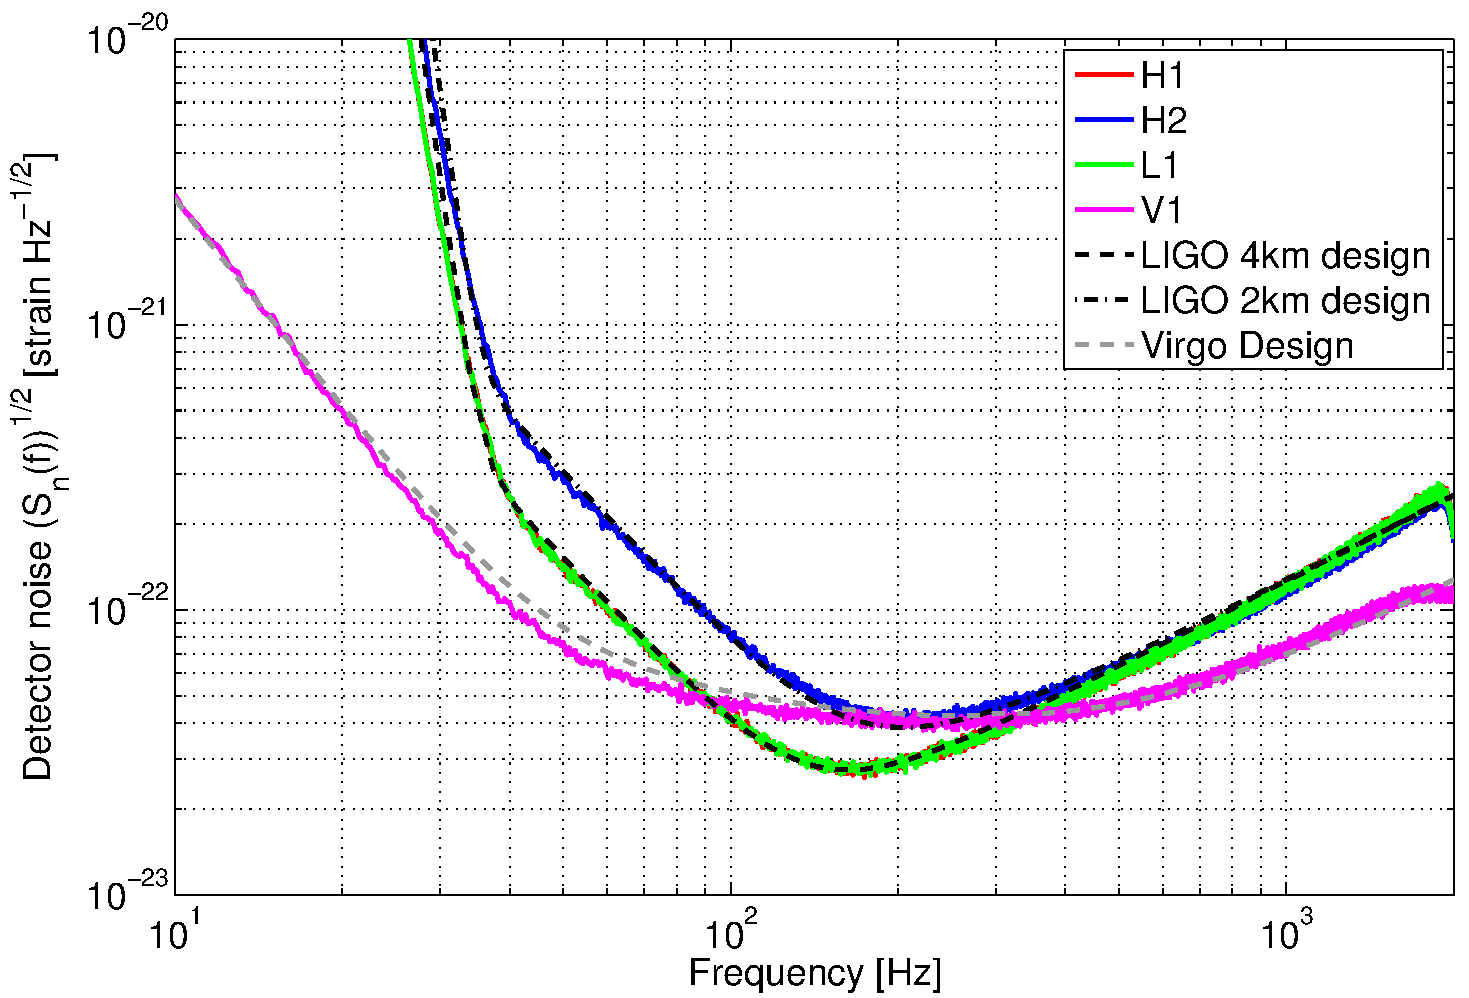
\includegraphics[width=\textwidth]{figures/ninja1/ninja_psd}
  \end{center}
  \caption[NINJA-1 noise curves]{
  \label{f:ninjapsd}
The NINJA data noise curves and the design spectra of the
 first generation LIGO and Virgo detectors.}
\end{figure}


We see from Figure~\ref{f:ninjapsd} that the noise power spectrum of
the NINJA data set closely approximates the Initial LIGO design
sensitivity in the frequency range of interest ($30$-$10^3\,$~Hz).
%The LIGO and Virgo data were generated using different techniques and
%software, and we note
There is a slight discrepancy with the Virgo design curve at low
frequencies (between approximately $20$ and $150\,$Hz), which is an
artefact of the Virgo noise generation procedure. Narrow-band features
such as the violin and mirror modes were removed from the detector
response used to compute the NINJA data, but were included in the
calculation of the Virgo design curve~\cite{PSD:VSR2}. The $1/f$ tails
of these narrow-band features are responsible for the small
discrepancy. 

Having generated the simulated detector data, we then generated a population of
simulated signals using the numerical relativity data.  This population was
constructed to cover a broad range of masses and signal amplitudes.  We
required that the starting frequency of the dominant $\ell=m=2$ mode of the
signal was not more than $30\,$Hz, an appropriate threshold given the
sensitivity curve of the Initial LIGO and Virgo detectors.  This sets a
minimum mass at which each waveform can be injected, which is given in Table
\ref{tab:allwaveforms-SI}. The minimum possible injection mass is therefore
$36 M_{\odot}$. The maximum mass was chosen as $350 M_{\odot}$.  To
get a good sample of long injected waveforms, we systematically chose a lower
range of masses for the longer waveforms. No restrictions were placed on the
other simulation parameters, i.e., the spins, mass-ratios and eccentricities. 
We ensured that waveforms from all the participating groups were equitably
represented by generating approximately 12 signals from the waveforms supplied
by each group. The time interval between adjacent injected signals was chosen
to be a random number in the range $700\pm 100\,$~s. 

Given these constraints, we generated the parameters of the signal
population.  The logarithm of the distance to the binary was drawn
from a uniform distribution ranging from $50\,$Mpc to $500\,$Mpc, and
the source locations and orientations were drawn from an isotropic
distribution of angles.  We then computed waveforms corresponding to
this population and at the appropriate sampling rate. We required that
the optimal matched filter signal-to-noise ratio of any injection be
greater than five in at least one of the four simulated detectors.
Any waveform that did not satisfy this constraint was discarded from
the population.  Subject to this condition, the distances of injected
signals varied from $52\,$Mpc to $480\,$Mpc (median at $145\,$Mpc),
the injected total mass range was $36M_\odot \le M \le346M_\odot$
(median at $155 M_\odot$), with individual component masses in the
range $11 M_\odot \le m_i \le193M_\odot$.  

Finally, the waveforms $h(t)$ were added to the simulated detector noise
$n(t)$ to generate the NINJA data set $s(t) = n(t) + h(t)$. As described
above, care was taken to ensure that signals were coherently injected in the
data streams from the four detectors.  The software for carrying out this
procedure is freely available as part of the LSC Algorithm Library
(LAL)~\cite{lal}.

The data set used in this analysis consisted of a total of 126 signals
injected in a total of 106 contiguous segments of noise each $1024\,$ s
long, thus spanning a duration of a little over $30\,$hours.
Figure~\ref{fig:distvsmass} shows the mass, spin and distance of the waveforms
contained in the NINJA data set.
\begin{figure}
  \begin{center}
  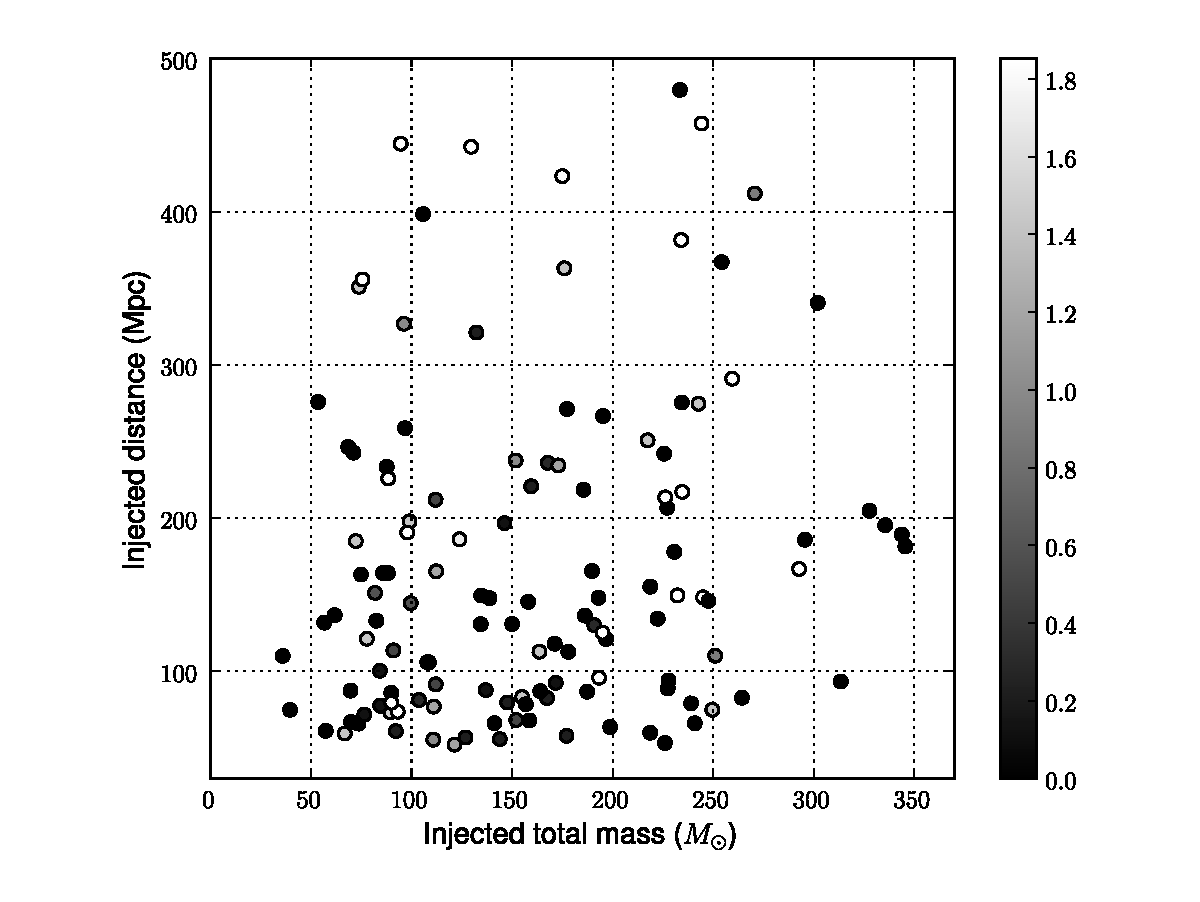
\includegraphics[width=0.9\textwidth]{figures/ninja1/DistanceVsMass_injected_withSpins}
  \end{center}
  \caption[Distribution of NINJA-1 injections]{The total mass and distance of the 126 NINJA injections. The
    grey scale encodes the sum of the dimensionless spins of the black holes, 
$|\vec{S_1}/m_1^2 + \vec{S_2}/m_2^2|$.}
  \label{fig:distvsmass}
\end{figure}


\section{Data Analysis Results}
\label{sec:ninja1_da}

Analysis of the NINJA-1 data was open to all and nine groups submitted
contributions using a variety of analysis techniques.  Participating
groups were provided with the NINJA-1 data set containing signals
embedded in noise and the parameters of the injected signals.
Analysts were not given access to the raw numerical-relativity
waveforms or noiseless injection data.

Methods used to analyse the NINJA-1 data include: matched-filter based
searches, un-modelled waveform searches using excess-power techniques,
and Bayesian model-selection and parameter-estimation techniques.
Where possible, the performance of different searches was compared.
The limited scope of the NINJA-1 data set makes detailed comparisons
difficult, however. 
%We plan to address
%this in future NINJA analyses.  
A list of the data-analysis contributions is shown in
Table~\ref{tab:ninja1_allda}. 
%
\begin{table}
\begin{center}
\begin{tabular}{|l|l|}\hline
Group & Analysis \\\hline
AEI & Phenomenological Waveforms in CBC pipeline \\
Birmingham & Bayesian Model Selection \\
Cardiff & Post-Newtonian (PN) Templates in CBC pipeline \\
Cardiff, Maryland & EOBNR waveforms in CBC pipeline \\
Goddard & Hilbert Huang Transform \\
Northwestern & Markov Chain Monte Carlo \\ 
Syracuse & Extended $\eta$ PN Templates in CBC pipeline \\
UMass, Urbino & Q-pipeline analysis \\
UWM & PN templates in CBC pipeline, Neyman-Pearson criteria \\
UWM, UMass, Urbino & Ringdown analysis \\
UWM, UMass, Urbino & Inspiral, Merger, Ringdown combined search  \\
\hline
\end{tabular}
\end{center}
\caption[The data-analysis contributions to the NINJA-1 project.]{
\label{tab:ninja1_allda}
The data-analysis contributions to the NINJA-1 project.}
\end{table}

\subsection{LIGO-only Searches}
\label{ssec:ninja1_ligo}

Henceforth we restrict attention to variations of the CBC pipeline,
described in chapter~\ref{ch:search}.  In particular, although many
variations of this pipeline were tested in NINJA-1, we focus on
testing the modifications to the template pN order, bank construction,
and termination frequency of the template waveforms suggested by the
comparison studies in chapter~\ref{ch:comparison}.  In this sense the
NINJA-1 project can be seen as an evolution of those studies; having
found a set of changes to the template waveforms that improve overlaps
with numeric signals, the next step is to test these changes in
searches.  The results of these searches are summarised in
Table~\ref{tab:inspiral_results}, each column giving the results from
a different search with a summary of the chosen parameters.  We first
describe the parameters varied between these analyses and then present
a more detailed discussion of the results.

All NINJA analyses using \emph{TaylorF2} waveforms (see Appendix A)
used restricted templates (i.e.~the amplitude is calculated to leading
order), however the phase was calculated to various different
post-Newtonian orders~\cite{Blanchet:2002av}. Phases were computed to
either two~\cite{Blanchet:1996pi,Blanchet:1995ez} or three point five
post-Newtonian
order~\cite{Blanchet:2001ax,PhysRevD.71.129902,Blanchet:2004ek} since
these are, respectively, the order used in LSC-Virgo
searches~\cite{Abbott:2009tt} as of the time of NINJA-1, and the
highest order at which post-Newtonian corrections are known.  The
studies in chapter~\ref{ch:comparison} show that 3.5 pN waveforms
provide better overlaps with numeric waveforms than 2.0 pN.

After choosing a post-Newtonian order, one chooses a region of
mass-parameter space to cover with the template bank.
Figure~\ref{f:ninjaBanks} shows the boundaries of the template banks
used in the analyses. One search used the range used by the LSC-Virgo
``low-mass'' search \cite{Abbott:2009tt} ($m_1,m_2 \ge  1 M_\odot, M
\le 35 M_{\odot}$) and all other searches used templates with total
masses in the range $20 M_\odot \le M \le 90 M_\odot$.  These
boundaries were chosen since there were no signals in the NINJA data
with mass smaller than $36 M_\odot$ and there is little, if any,
inspiral power in the sensitive band of the NINJA data for signals
with $M \gtrsim 100 M_\odot$.

The standard LSC-Virgo template bank generation
code~\cite{Babak:2006ty} restricts template generation to signals with
$\eta \le 0.25$, since it is not possible to invert $M$ and $\eta$ to
obtain real-valued component masses for $\eta > 0.25$.  All but one of
the searches enforced this constraint, with the $0.03 \le \eta \le
0.25$ for the low-mass CBC search and $0.1 \le \eta \le 0.25$ for the
other ``physical-$\eta$'' searches.  However, the comparison studies
show that the overlaps obtain maximum values at unphysical values of
$\eta$ over much of the mass space.  In particular, with 3.5 pN
waveforms unphysical $\eta$ values provide better overlaps above
$40 \msun$, which is the mass range covered by the NINJA-1 injections.
However, these studies allowed allowed the values to vary continuously
and did not take into account the discretization imposed by a template
bank, nor the parameter coincidence required at the second stage of
the pipeline.  It is therefore critical to test the extended $\eta$
bank in searches.

Finally, it is necessary to specify a frequency at which to terminate
the TaylorF2 waveform. In the LSC-Virgo analyses, this is chosen to be
the innermost stable circular orbit (ISCO) frequency for a test mass
in a Schwarzschild spacetime 
%
\begin{equation} \label{f_ISCO} f_\mathrm{ISCO} =
\frac{c^3}{6\sqrt{6}\pi GM}.  \end{equation}
%
This cutoff was chosen as the point beyond which the TaylorF2
waveforms diverge significantly from the true evolution of the
binary~\cite{Blanchet:2002av}.  However, the studies reported in
chapter~\ref{ch:comparison} as well as those in~\cite{Pan:2007nw} have
shown that extending the waveforms up to higher frequencies improves
the sensitivity of TaylorF2 templates to higher mass signals.  The
NINJA-1 TaylorF2 analyses use templates terminated at the ISCO
frequency and two additional cut-off frequencies: the effective
ringdown (ERD) frequency and a weighted ringdown ending (WRD)
frequency. The ERD frequency was obtained by comparing post-Newtonian
models to the Pretorius and Goddard waveforms~\cite{Pan:2007nw}. The
ERD almost coincides with the fundamental quasi-normal mode frequency
of the black hole formed by the merger of an equal-mass non-spinning
black-hole binary. The weighted ringdown ending (WRD) frequency is
lies between ISCO and ERD, and found to close to optimal in
chapter~\ref{ch:comparison}.  It is calculated as in
Eqn.~\ref{eq:fCut}


\begin{landscape}
\begin{table}
\begin{center}
\begin{tabular}{| l || c | c | c | c | c | c | c |}
\hline
\bf{Analysis} \T \B & $(1)$ & $(2)$ & $(3)$ & $(4)$ & $(5)$ & $(6)$ \\ \hline
\bf{Freq. Cutoff} \T \B & ISCO & ISCO & ERD & ERD &  WRD & WRD  \\ 
\hline
\bf{PN Order} & 2 PN & 2 PN & 2 PN & 3.5 PN &  3.5 PN& 3.5 PN  \\
\hline
%\parbox{2.8cm}{
%\bf{Component\\ Mass $M_{\odot}$}} & 1--34 & 10--60 & 10--60 & 10--60 & 10--60 & 10--60 \\ 
%\hline
\bf{Total Mass $M_{\odot}$} \T \B & 2--35 & 20--90 & 20--90 & 20--90 & 20--90 & 20--90  \\ 
\hline
\bf{$\eta$ range} \T \B & 0.03--0.25 & 0.10--0.25 & 0.10--0.25 & 0.10--0.25 & 0.10--0.25 & 0.10--1  \\ 
\hline
\bf{Found Single (H1, H2, L1)}\TT \BB  & 69, 66, 75 & 72, 43, 66 & 83, 51, 81 & 91, 56, 87 & 90, 55, 88 & 90, 56, 88 \\ 
\hline
\bf{Found Coincidence } \TT \BB & 49 & 59 & 79 & 82 &  82 & 84 \\ 
\hline
\bf{Found Second Coincidence} \TT \BB & 48 & 59 & 77 & 81 &  81 & 81 \\ 
\hline 
\end{tabular}
\caption[Results of inspiral searches using TaylorF2 templates.] {
\label{tab:inspiral_results}
Results of inspiral searches using TaylorF2 templates.  There were 126
injections performed into the data.  The table above shows the number of
injections which were recovered from the three simulated LIGO detectors
(H1, H2 and L1) using various different waveform families, termination frequencies
$f_\mathrm{ISCO}$, $f_\mathrm{ERD}$ and $f_\mathrm{WRD}$ 
(as described in the text), and post-Newtonian orders.} 
\end{center}
\end{table}
\end{landscape}

\begin{figure}
  \begin{center}
  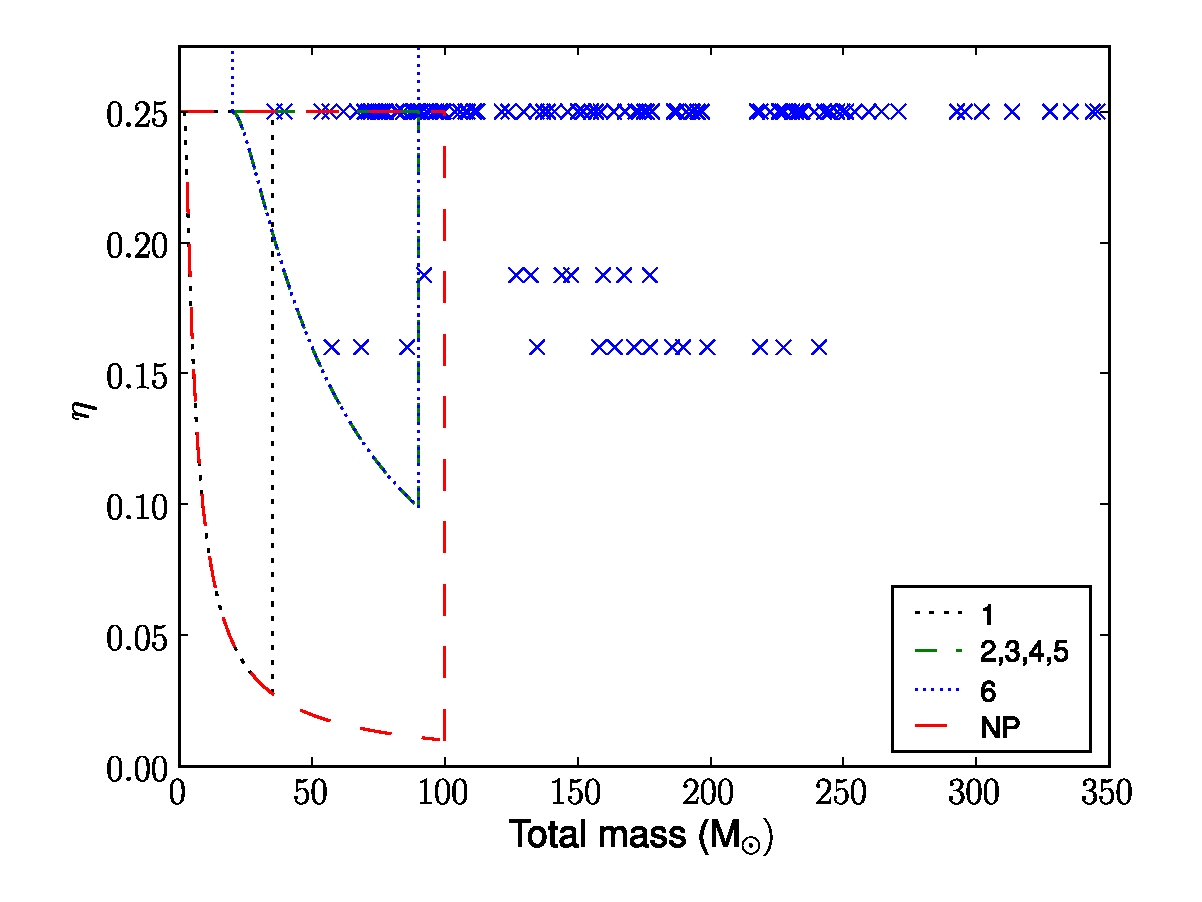
\includegraphics[width=0.8\textwidth]{figures/ninja1/ninja_banks}
  \end{center}
  \caption[Boundaries of template banks in NINJA-1 inspiral searches]{
\label{f:ninjaBanks}
Boundaries of the template banks used in inspiral searches as a
function of total mass $M$ and symmetric mass ratio $\eta$. The crosses show
the location of the injections in the NINJA data set. The numbers in the
legend correspond to entries in table~\ref{tab:inspiral_results}. Bank 6
extends in a rectangle up to $\eta = 1.00$, as indicated by the arrows. NP
is the bank used in the Neyman-Pearson analysis not covered here.}
\end{figure}

The results of these searches are reported in
Table~\ref{tab:inspiral_results}.  The principal result is the number
of injected signals detected by the search.  For simplicity, we define
a detected signal as one for which there is a candidate
gravitational-wave signal observed within $50$~ms of the coalescence
time of the injection, determined by the maximum gravitational-wave
strain of the injected signal.  We do not impose any additional
threshold on the measured SNR or effective SNR of the candidate.  For
a single detector, this will lead to a small number of falsely
identified injections, but for coincidence results the false alarm
rate is so low that we can be confident that the triggers are
associated with the injection. We now describe these results in the
order that they appear in Table~\ref{tab:inspiral_results}.

Search~$(1)$ used second order post-Newtonian templates terminated at
$f_\mathrm{ISCO}$ with a maximum mass of $M \le 35 M_{\odot}$.
Despite the fact that no NINJA injections had a mass within the range
of this search, a significant number of signals were still recovered
in coincidence both before and after signal consistency tests.
Although the templates are not a particularly good match to the
injected signals, they are still similar enough to produce triggers at
the time of the injections.  Search~$(2)$ changed the boundary of the
template bank to $20 M_\odot \le M \le 90 M_{\odot}$, but left all
other parameters unchanged.  The number of detected signals increases
significantly as more signals now lie within the mass range searched. 

Search~$(3)$ extended the upper cutoff frequency of the waveforms to
$f_\mathrm{ERD}$. The number of signals detected increased from 59 to
77, as expected since these waveforms can detect some of the power
contained in the late inspiral or early merger part of the
signal~\cite{Pan:2007nw,Boyle:2009dg}. Search~$(4)$ extends the
post-Newtonian order to 3.5~PN, slightly increasing the number of
detected signals to 81.  With the limited number of simulations
performed in this first NINJA analysis, it is difficult to draw a
strong conclusion, although there does seem to be evidence that the
higher post-Newtonian order waveforms perform better, consistent with
previous comparisons of post-Newtonian and numerical relativity
waveforms
\cite{Pan:2007nw,Baker:2006ha,Hannam:2007ik,Boyle:2008ge,Boyle:2009dg}
and chapter~\ref{ch:comparison}.

Search~$(5)$ uses an upper-frequency cutoff of $f_\mathrm{WRD}$ for
the templates. The number of injections found in coincidence for this
search is the same as the search using $3.5$ order templates with a
cutoff of $f_\mathrm{ERD}$, although there are slight differences in
the number of found injections at the single detector level.

Search~$(6)$ extends the template bank of search~$(5)$ to unphysical
values of the symmetric mass ratio. Extending the bank to $\eta\le 1$
increases the number of templates in the bank by a factor of $\sim 2$.
The original and modified template banks are shown in
Figure~\ref{f:templateBanks}. With the extended template bank the
number of injections found in coincidence remains the same as
search~$(5)$ after signal-based vetoes are applied.  However, many of
the injections are recovered at a higher SNR, particular the low-mass
signals, as shown in Figure~\ref{f:templateBanks}.  Some injections
show a reduction in SNR; more work is needed to understand this
effect.

\begin{figure}
  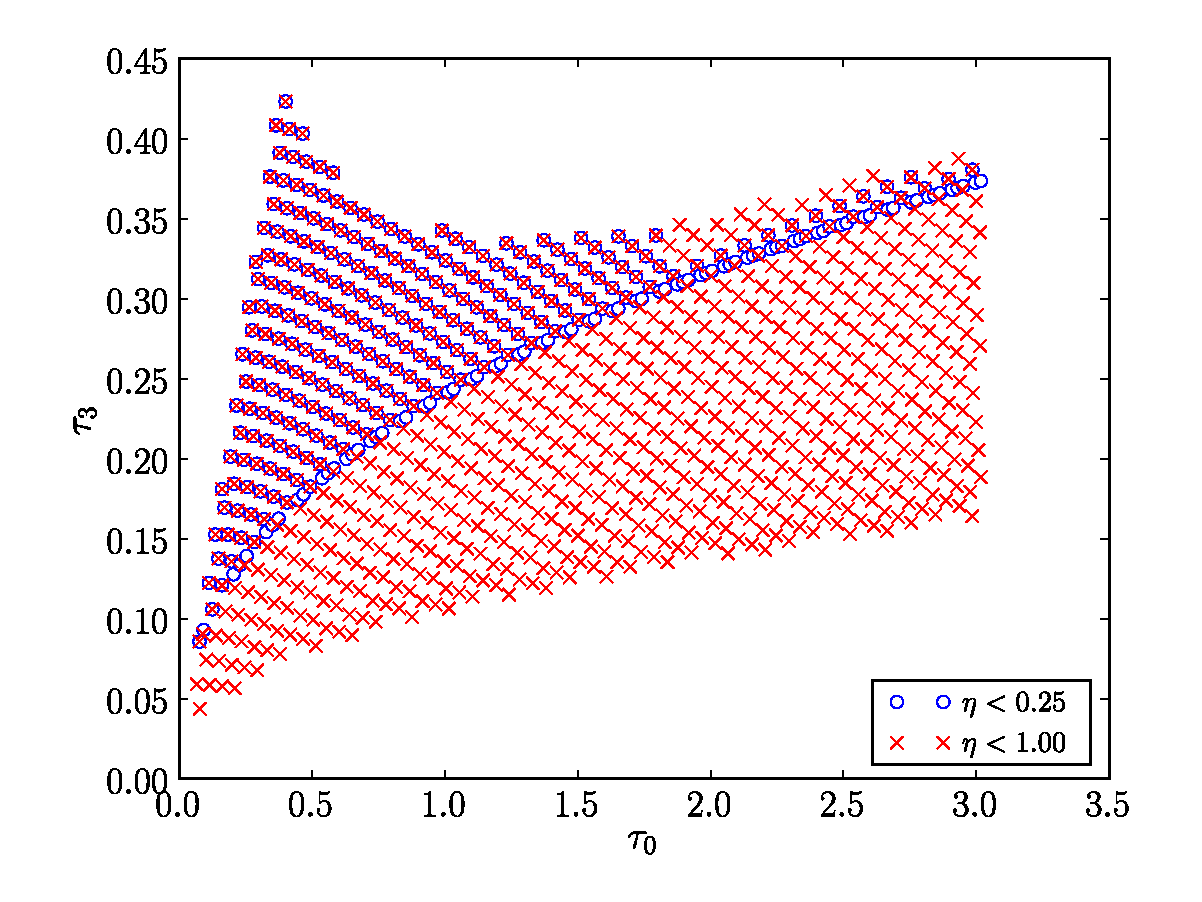
\includegraphics[width=0.50\textwidth]{figures/ninja1/BankBoth}
  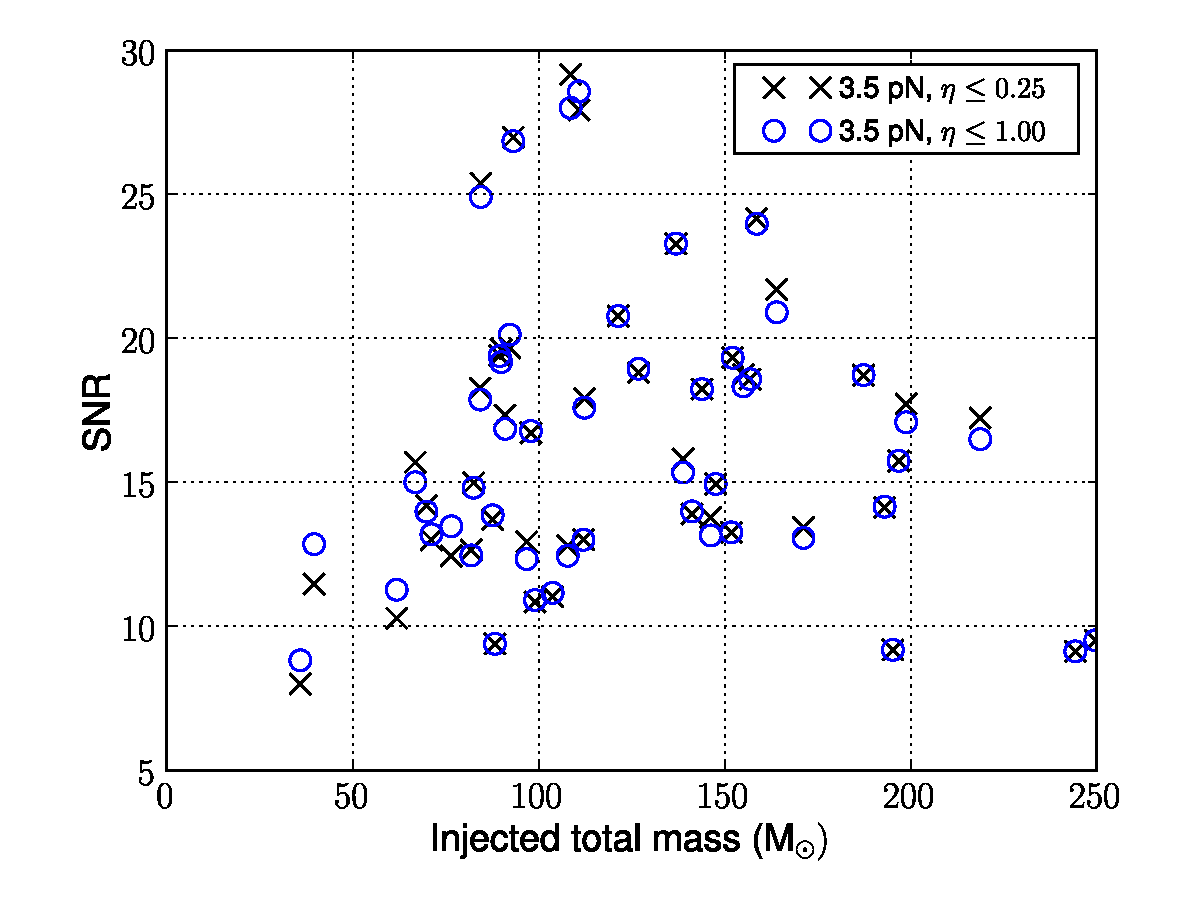
\includegraphics[width=0.50\textwidth]{figures/ninja1/HanfordSNR}
  \caption[NINJA-1 results from the extended template bank]{
  {\bf Left:} The template bank generated by the LSC-Virgo
  search pipeline (circles) and the bank obtained by extending to
  $\eta \leq 1.00$ (crosses). In this figure the bank is parametrised
  by $\tau_0$ and $\tau_3$ which are related to the binary masses by
  $\tau_0 = 5M/(256\eta v_0^8)$ and $\tau_3 = \pi M/(8\eta v_0^5)$,
  where $v_0 = (\pi M f_0)^{1/3}$ is a fiducial velocity parameter
  corresponding to a fiducial frequency $f_0 = 40.0 Hz$.
  {\bf Right:} The
  signal-to-noise (SNR) ratio at which NINJA injections were recovered using
  the $\eta \le 0.25$ bank (squares) and the $\eta \le 1$ extended bank
  (circles) in the Hanford detectors, given by $\rho =
  (\rho_\mathrm{H1}^2 + \rho_\mathrm{H2}^2)^{1/2}$. The SNR of the signal
  recovered using the extended bank shows with significant ($> 10\%$) 
  increases over the standard bank for certain injections.}
  \label{f:templateBanks}
\end{figure}

Finally, we note that the majority of signals passed the $\chi^2$
signal-based veto with the thresholds used in the LSC-Virgo pipeline.  The
last two lines of Table~\ref{tab:inspiral_results} show the number of
recovered signals before and after these signal-based vetoes are
performed. The post-Newtonian templates and numerical relativity signals are
similar enough that virtually all of the injected signals survive the signal
based vetoes. 

To illustrate the results of these analyses in more detail, 
Figure~\ref{fig:3_5pn_found_missed} shows which signals were detected and which were
missed by the 3.5 order post-Newtonian TaylorF2 templates terminated at
$f_\mathrm{ERD}$, as a function of injected
total mass and effective distance of the binary (a measure of the
amplitude of the signal in the detector), defined by~\cite{Allen:2005fk}
\begin{equation}
D_\mathrm{eff} = d \left/ \sqrt{F_+^2 (1 + \cos^2 \iota)^2/4 + F_\times^2 \cos^2 \iota}\right.,
\label{eq:effdist}
\end{equation}
where $d$ is the luminosity distance of the binary.

One signal, with total mass of $110 M_{\odot}$ and effective distance
$\sim 200$ Mpc, was missed while others with similar parameters were
found.  This signal was one of the Princeton waveforms (labelled
\verb|PU-e0.5| in Figure \ref{fig:NR-Reh22}) for which the maximum
amplitude occurs at the start of the waveform rather than at
coalescence\footnote{That the maximum occurs at the start of the
waveform is in part an ``artifact'' of the double-time integration
from the Newman-Penrose scalar $\psi_4$ to the metric perturbation
$h$, and in part a coordinate artifact.  The two integration constants
were chosen to remove a constant and linear-in-time piece for $h$,
however, there is still a non-negligible quadratic component; we {\em
suspect} this is purely gauge, though lacking a better understanding
of this it was not removed from the waveform.}, rendering our simple
coincidence test invalid.  The injection finding algorithm compares
the peak time to the trigger time and, even though triggers are found
at the time of the simulation, there are no triggers within the
$50$~ms window used to locate detected signals.

\begin{figure}
\begin{center}
  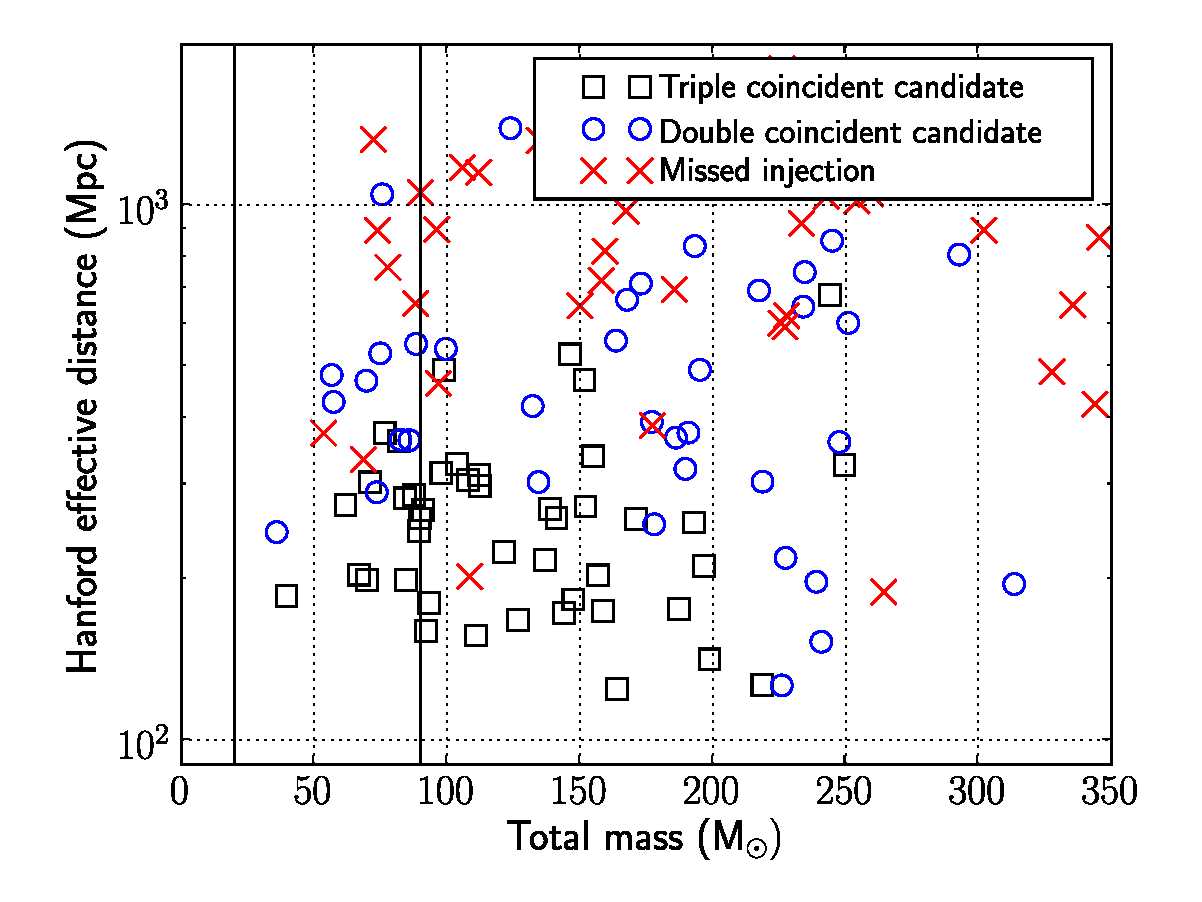
\includegraphics[width=0.49\textwidth]{figures/ninja1/spa_erd_3_5pn_found_missed_mchirp}
  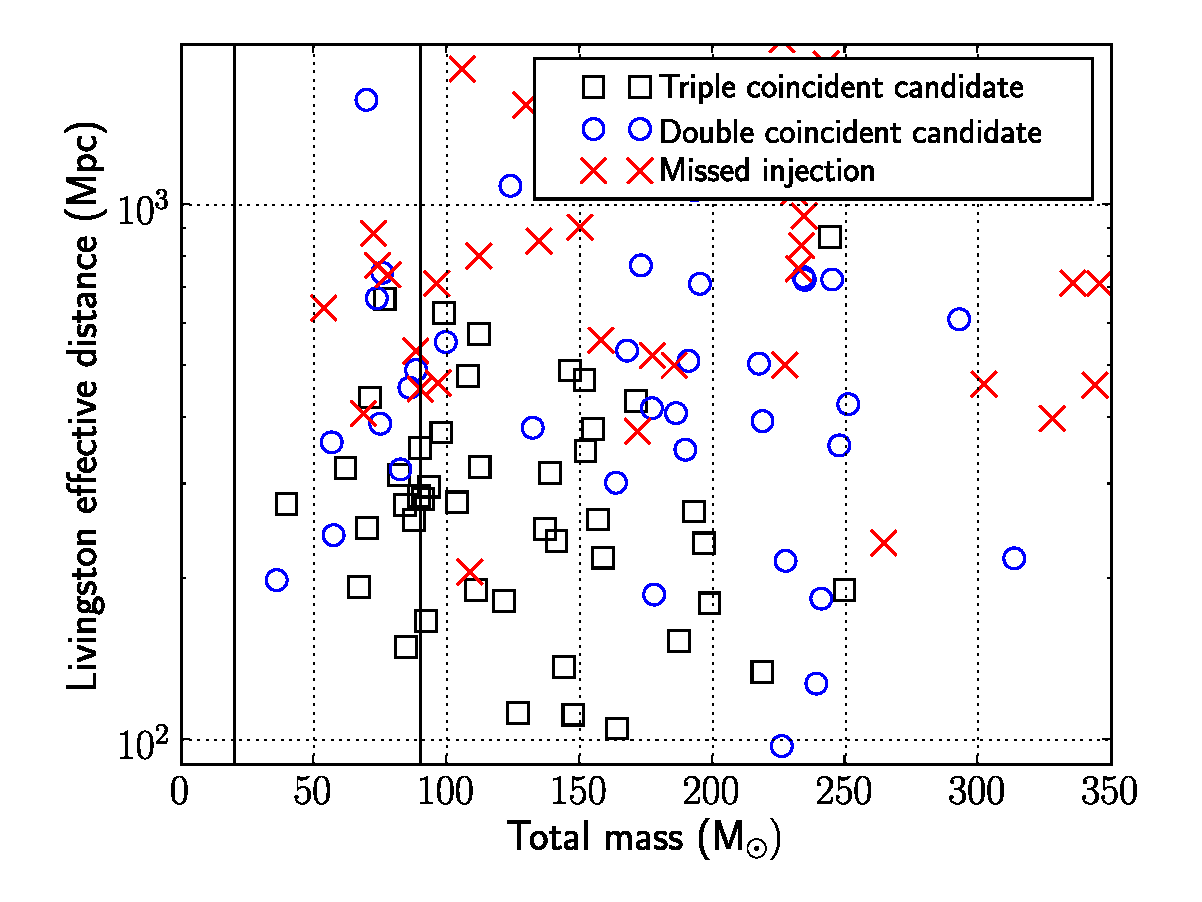
\includegraphics[width=0.49\textwidth]{figures/ninja1/spa_erd_3_5pn_found_missed_mchirp_l}
\end{center}
\caption[NINJA-1 injections found/missed by an inspiral search with
$f_c=$ ERD.]{
\label{fig:3_5pn_found_missed}
Found and missed injections using TaylorF2 templates
terminated at ERD, plotted as a function of the injected effective
distance in Hanford (left) and Livingston (right) and the total mass
of the injection. Since the LIGO Observatories are not exactly
aligned, the effective distance of a signal can differ, depending on
the sky location of the signal.  The vertical bars mark the limits of
the template bank used in the search.  For the lower masses, we see
that the majority of the closer injections are found in coincidence in
all three of the detectors.  There is then a band of injections which
are found only in two detectors -- H1 and L1 and not the less
sensitive H2 detector.  For higher masses, the results are less
meaningful as the template bank was only taken to a total mass of $90
M_{\odot}$.}
\end{figure}

Figure~\ref{fig:3_5pn_params} shows the accuracy with which the total mass and
coalescence time of the binary are recovered when using the 3.5 post-Newtonian
order Taylor F2 templates. The total mass fraction difference is computed as
$(M_\mathrm{injected} - M_\mathrm{detected})/ M_\mathrm{injected}$. For lower
mass signals, the end time is recovered reasonably accurately, with accuracy
decreasing for the high mass systems. The total mass recovery is poor for the
majority of signals, with good parameter estimation for only a few of the
lowest mass simulations.

\begin{figure}
    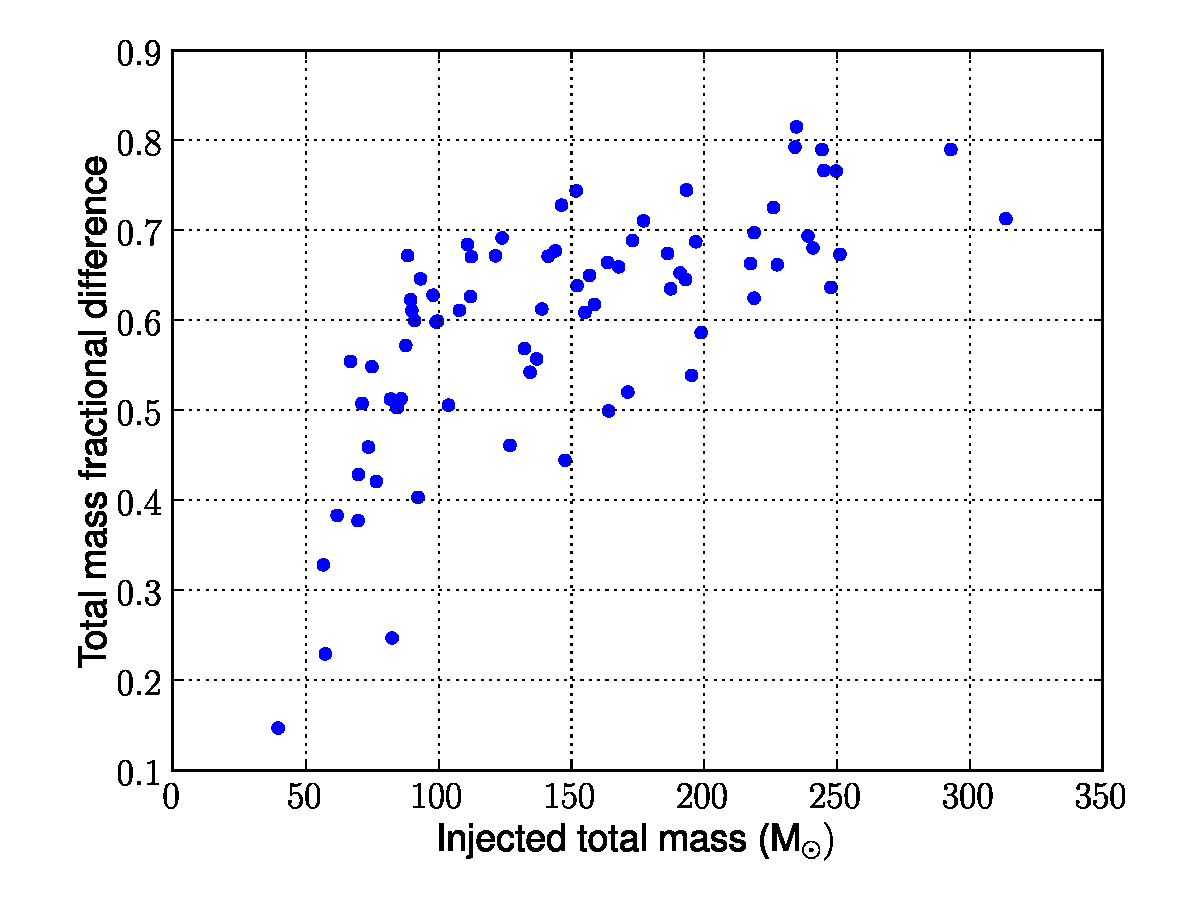
\includegraphics[width=0.50\textwidth]{figures/ninja1/spa_erd_3_5pn_mass_estimate}
    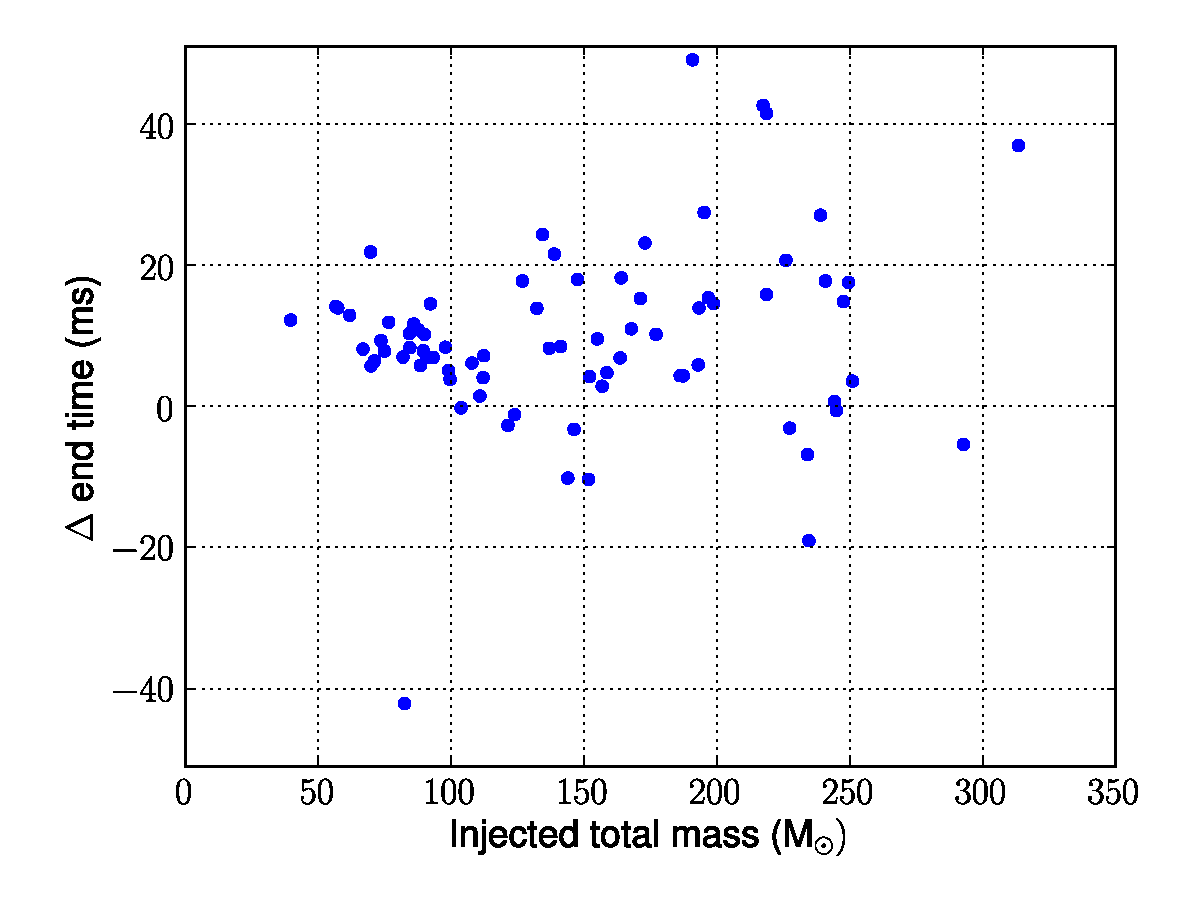
\includegraphics[width=0.50\textwidth]{figures/ninja1/spa_erd_3_5pn_time_estimate_vs_mt}
\caption[Parameter accuracy using TaylorF2 templates terminated at ERD]{
\label{fig:3_5pn_params}
Parameter accuracy using TaylorF2 templates terminated at
ERD.\textbf{Left:} Accuracy with which the total mass is recovered. The
template bank covers the region $20 M_\odot \le M \le 90 M_\odot$, hence
the mass of injections with $M > 90 M_\odot$ are always underestimated.
Even within the region covered by the bank, the TaylorF2 templates
systematically underestimate the mass of the injected signals and the total
mass is recovered accurately only for a few injections.  The vast majority of
recovered signals have an error of $40\%$ or greater. \textbf{Right:} Accuracy
of determining the coalescence time of the injections.  The end time is not
recovered accurately, the timing error can become as large as $50
\mathrm{ms}$, the limits of the injection window.}
\end{figure}

% end inspiral_templates.tex


\section{Conclusion}
%\label{sec:discussion}
%\input{discussion}

We have applied the alterations to the inspiral templates and bank
suggested by the studies of the previous chapter to search for NR
signals injected into Gaussian noise as part of the NINJA-1 project.
The results indicate that these alterations are indeed advantageous.
In particular, the second and last columns of
table~\ref{tab:inspiral_results} compare the pipeline used in the S5
search (with a mass range extended to cover the range of injections)
to the pipeline with all our recommendations implemented.  By
implementing these changes we recover approximately 25\% more
injections.

However, NINJA-1 took an open policy towards NR submissions and
consequently there may be issues with the waveforms that limit our
ability to draw definitive conclusions.  The lower limit on mass at
which waveforms could be injected certainly limits our ability to make
statements on a low-mass search.

In order to refine these results it will be necessary to use longer
waveforms that have been subjected to more rigorous validation.  This
is the goal of the second NINJA project, discussed in the next
chapter.

